% !TEX program = pdflatex
% !TEX encoding = UTF-8 Unicode

% Plantilla de la clase `scrbook` del paquete KOMA-script para la
% elaboración de un TFG siguiendo las directrices del la comisión del
% Grado en Matemáticas de la Universidad de Granada.

% Francisco Torralbo Torralbo
% miércoles, 29 de abril de 2020

\documentclass{scrbook}

\KOMAoptions{%
  fontsize=10pt,        % Tamaño de fuente
  paper=a4,             % Tamaño del papel
  headings=normal,      % Tamaño de letra para los títulos: small, normal, big
  % parskip=half,         % Espacio entre párrafos: full (una línea) o half (media línea)
  headsepline=false,    % Una linea separa la cabecera del texto
  cleardoublepage=empty,% No imprime cabecera ni pie en páginas en blanco 
  chapterprefix=false,  % No antepone el texto "capítulo" antes del número
  appendixprefix=false,	% No antepone el texto "Apéndice" antes de la letra
  listof=totoc,		    	% Añade a la tabla de contenidos la lista de tablas y figuras
  index=totoc,			    % Añade a la talba de contenidos una entrada para el índice
  bibliography=totoc,	  % Añade a la tabla de contenidos una entrada para bibliografía
  BCOR=5mm,           % Reserva margen interior para la encuadernación. 
                        % El valor dependerá el tipo de encuadernado y del grosor del libro.
  DIV=10,             % Cálcula el diseño de página según ciertos 
                        % parámetros. Al aumentar el número aumentamos el ancho de texto y disminuimos el ancho del margen. Una opción de 14 producirá márgenes estrechos y texto ancho.
}

% INFORMACIÓN PARA LA VERSIÓN IMPRESA
% Si el documento ha de ser impreso en papel de tamaño a4 pero el tamaño del documento (elegido en \KOMAoptions con la ocpión paper) no es a4 descomentar la línea que carga el paquete `crop` más abajo. El paquete crop se encargará de centrar el documento en un a4 e imprimir unas guías de corte. El procedimiento completo para imprenta sería el siguiente:
% 0. Determinar, según el tipo de encuadernación del documento, el ancho reservado para el proceso de encuadernación (preguntar en la imprenta), es decir, la anchura del área del papel que se pierde durante el proceso de encuadernación. Fijar la varibale BCOR de \KOMAoptions a dicho valor.
% 1. Descomentar la siguiente línea e imprimir una única página con las guías de corte
% 2. Cambiar la opción `cross` por `cam` (o `off`) en el paquete crop y volver a compilar. Imprimir el documento (las guías de corte impresas no inferfieren con el texto).
% 3. Usar la página con las guías impresas en el punto 1 para cortar todas las páginas.

% \usepackage[a4, odd, center, pdflatex, cross]{crop} % Permite imprimir el documento en un a4 (si el tamaño es más pequeño) mostrando unas guías de corte. Útil para imprenta.

% VERSIÓN ELECTRÓNICA PARA TABLETA
% Las opciones siguientes seleccionan un tamaño de impresión similar a una tableta de 9 pulgadas con márgenes estrechos. Útil para producir una versión en pdf para ser leída en una tableta en lugar de impresa.
% Para que la portada quede centrada correctamente hay que editar el
% archivo `portada.tex` y eliminar el entorno `addmargin`

% \KOMAoptions{fontsize=10pt, paper=19.7104cm:14.7828cm, twoside=false, BCOR=0cm, DIV=14}

% ---------------------------------------------------------------------
%	PAQUETES 
% ---------------------------------------------------------------------

% CODIFICACIÓN E IDIOMA
% ---------------------------------------------------------------------
\usepackage[utf8]{inputenc} 			    % Codificación de caracteres

% Selección del idioma: cargamos por defecto inglés y español (aunque este último es el idioma por defecto para el documento). Cuando queramos cambiar de idioma escribiremos:
% \selectlanguage{english} o \selectlanguage{spanish}

\usepackage[english, spanish, es-nodecimaldot, es-noindentfirst, es-tabla]{babel}

% Opciones cargadas para el paquete babel:
  % es-nodecimaldot: No cambia el punto decimal por una coma en modo matemático.
  % es-noindentfirst: No sangra los párrafos tras los títulos.
  % es-tabla: cambia el título del entorno `table` de "Cuadro" a "Tabla"

% Otras opciones del paquete spanish-babel:
  \unaccentedoperators % Desactiva los acentos en los operadores matemáticso (p.e. \lim, \max, ...). Eliminar esta opción si queremos que vayan acentuados

% MATEMÁTICAS
% ---------------------------------------------------------------------
\usepackage{amsmath, amsthm, amssymb} % Paquetes matemáticas
\usepackage{mathtools}                % Añade mejoras a amsmath
\mathtoolsset{showonlyrefs=true}      % sólo se numeran las ecuaciones que se usan
\usepackage[mathscr]{eucal} 					% Proporciona el comando \mathscr para
                                      % fuentes de tipo manuscrito en modo matemático sin sobreescribir el comando \mathcal

% TIPOGRAFÍA 
% ---------------------------------------------------------------------
% El paquete microtype mejora la tipografía del documento.
\usepackage[activate={true,nocompatibility},final,tracking=true,kerning=true,spacing=true,factor=1100,stretch=10,shrink=10]{microtype}

% Las tipografías elegidas para el documento, siguiendo la guía de estilo de la UGR,
% son las siguientes
% Normal font: 			URW Palladio typeface. 
% Sans-serif font: 	Gill Sans
% Monospace font: 	Inconsolata
\usepackage[T1]{fontenc}
\usepackage[sc, osf]{mathpazo} \linespread{1.05}         
\usepackage[scaled=.95,type1]{cabin} % sans serif in style of Gill Sans
% Si el paquete cabin da error usar el siguiente comando en su lugar
% \renewcommand{\sfdefault}{iwona} 
\usepackage{inconsolata}


% Selecciona el tipo de fuente para los títulos (capítulo, sección, subsección) del documento.
\setkomafont{disposition}{\sffamily\bfseries}

% Cambia el ancho de la cita. Al inicio de un capítulo podemos usar el comando \dictum[autor]{cita} para añadir una cita famosa de un autor.
\renewcommand{\dictumwidth}{0.45\textwidth} 

\recalctypearea % Necesario tras definir la tipografía a usar.

% TABLAS, GRÁFICOS Y LISTADOS DE CÓDIGO
% ---------------------------------------------------------------------
\usepackage{booktabs}
% \renewcommand{\arraystretch}{1.5} % Aumenta el espacio vertical entre las filas de un entorno tabular

\usepackage{xcolor, graphicx}
% Carpeta donde buscar los archivos de imagen por defecto
\graphicspath{{img/}}

% IMAGEN DE LA PORTADA
% Existen varias opciones para la imagen de fondo de la portada del TFG. Todas ellas tienen en logotipo de la universidad de Granada en la cabecera. Las opciones son las siguientes:
% 1. portada-ugr y portada-ugr-color: diseño con marca de agua basada en el logo de la UGR (en escala de grises y color).
% 2. portada-ugr-sencilla y portada-ugr-sencilla-color: portada únicamente con el logotipo de la UGR en la cabecera.
\usepackage{eso-pic}
\newcommand\BackgroundPic{%
	\put(0,0){%
		\parbox[b][\paperheight]{\paperwidth}{%
			\vfill
			\centering
      % Indicar la imagen de fondo en el siguiente comando
			
\includegraphics[width=\paperwidth,height=\paperheight,%
			keepaspectratio]{portada-ugr-sencilla}%
			\vfill
}}}

% \usepackage{listings} % Para la inclusión de trozos de código

% CABECERAS
% ---------------------------------------------------------------------
% Si queremos modificar las cabeceras del documento podemos usar el paquete
% `scrlayer-scrpage` de KOMA-Script. Consultar la documentación al respecto.
% \usepackage[automark]{scrlayer-scrpage}

% VARIOS
% ---------------------------------------------------------------------

%\usepackage{showkeys}	% Muestra las etiquetas del documento. Útil para revisar las referencias cruzadas.

% ÍNDICE 
% Para generar el índice hay que compilar el documento con MakeIndex. Generalmente los editores se encargan de ello automáticamente.
% ----------------------------------------------------------------------
% \index{} para añadir un elemento
% \index{main!sub} para añadir un elementos "sub" bajo la categoría "main".
% \index{termino|textbf} para dar formato al número de página (negrita).
% \index{termino|see{termino relacionado}} para crear una referencia cruzada

% Ejemplo: \index{espacio homogéneo}, \index{superficie!mínima}, \index{esfera|see{espacio homogéneo}}

\usepackage{makeidx}
%\usepackage{showidx} % Muestra en el margen del documento las entradas añadidas al índice. Útil para revisar el documento. Si está activo el índice no se genera
\makeindex

% ---------------------------------------------------------------------
% COMANDOS Y ENTORNOS
% ---------------------------------------------------------------------
% Cargamos un archivo externo donde hemos incluido todos los comandos
% propios que vamos a usar en el documento.
% DEFINICIÓN DE COMANDOS Y ENTORNOS

% CONJUNTOS DE NÚMEROS

  \newcommand{\N}{\mathbb{N}}     % Naturales
  \newcommand{\R}{\mathbb{R}}     % Reales
  \newcommand{\Z}{\mathbb{Z}}     % Enteros
  \newcommand{\Q}{\mathbb{Q}}     % Racionales
  \newcommand{\C}{\mathbb{C}}     % Complejos

% TEOREMAS Y ENTORNOS ASOCIADOS

  % \newtheorem{theorem}{Theorem}[chapter]
  \newtheorem*{teora}{Teorema A}
  \newtheorem*{teorb}{Teorema B}
  \newtheorem*{teorema*}{Teorema}
  \newtheorem{teorema}{Teorema}[chapter]
  \newtheorem{proposicion}{Proposición}[chapter]
  \newtheorem{lema}{Lema}[chapter]
  \newtheorem{corolario}{Corolario}[chapter]
  \newtheorem{hecho}{Hecho}[chapter]

    \theoremstyle{definition}
  \newtheorem{definicion}{Definición}[chapter]
  \newtheorem{ejemplo}{Ejemplo}[chapter]

    \theoremstyle{remark}
  \newtheorem{observacion}{Observación}[chapter]


% --------------------------------------------------------------------
% INFORMACIÓN DEL TFG Y EL AUTOR
% --------------------------------------------------------------------
\usepackage{xspace} % Para problemas de espaciado al definir comandos

\newcommand{\miTitulo}{Estructuras diferenciables sobre una superficie topológica y la visualización computacional de superficies.\xspace}
\newcommand{\miNombre}{Norberto Fernández de la Higuera\xspace}
\newcommand{\miGrado}{Doble Grado en Ingeniería Informática y Matemáticas}
\newcommand{\miFacultad}{Facultad de Ciencias}
\newcommand{\miUniversidad}{Universidad de Granada}
% Añadir tantos tutores como sea necesario separando cada uno de ellos
% mediante el comando `\\\medskip` y una línea en blanco
\newcommand{\miTutor}{
  Francisco José López Fernández \\ \emph{Departamento de Geometría y Topología} 

  % Añadir tantos tutores como sea necesario. 
  \medskip
  Carlos Ureña Almagro \\ \emph{Departamento de Lenguajes y Sistemas Informáticos}
}
\newcommand{\miCurso}{2020-2021\xspace}

% HYPERREFERENCES
% --------------------------------------------------------------------
\usepackage{xurl}
\usepackage[pagebackref]{hyperref}
% Opciones para el paquete hyperref
%----------------------------------

\hypersetup{%
  % hidelinks,            % Enlaces sin color ni borde. El borde no se imprime
  linkbordercolor=0.8 0 0,
  citebordercolor=0 0.8 0,
  citebordercolor=0 0.8 0,
  colorlinks = true,            % Color en texto de los enlaces. Comentar esta línea o cambiar `true` por `false` para imprimir el documento.
  linkcolor = [rgb]{0.5, 0, 0}, % Color de los enlaces internos
  urlcolor = [rgb]{0, 0, 0.5},  % Color de los hipervínculos
  citecolor = [rgb]{0, 0.5, 0}, % Color de las referencias bibliográficas
	pdftitle={\miTitulo},%
	pdfauthor={\textcopyright\ \miNombre, \miFacultad, \miUniversidad},%
  pdfsubject={Trabajo de fin de Grado},%
	pdfkeywords={},%
	pdfcreator={pdfLaTeX},%
}

% Redefinición del estilo para mostrar las referencias cruzadas en la bibliografía.
\renewcommand*{\backref}[1]{}
\renewcommand*{\backrefalt}[4]{{\footnotesize [%
    \ifcase #1 No citado%
    \or Citado en pág.~#2%
    \else Citado en págs. #2%
    \fi%
]}}

% Etiquetas en español para el comando \autoref
\def\chapterautorefname{Capítulo}
\def\appendixautorefname{Apéndice}
\def\sectionautorefname{Sección}
\def\subsectionautorefname{Subsección}
\def\figureautorefname{Fig.}
\def\tableautorefname{Tabla}

\def\teoremaautorefname{Teorema}
\def\proposicionautorefname{Proposición}
\def\lemaautorefname{Lema}
\def\corolarioautorefname{Corolario}
\def\definicionautorefname{Def.}
\def\observacionautorefname{Observación}
\def\ejemploautorefname{E.j.}

% Pone automáticamente un parántesis para las ecuaciones
\def\equationautorefname~#1\null{Ec.~(#1)\null}


\begin{document}

% --------------------------------------------------------------------
% FRONTMATTER
% -------------------------------------------------------------------
\frontmatter % Desactiva la numeración de capítulos y usa numeración romana para las páginas

% \pagestyle{plain} % No imprime cabeceras

% !TeX root = ../libro.tex
% !TeX encoding = utf8

%*******************************************************
% Titlepage
%*******************************************************
\begin{titlepage}
  \AddToShipoutPicture*{\BackgroundPic}
  \phantomsection 
  \pdfbookmark[1]{Título}{title}

  % Para que el título esté centrado en la página.
  % Los valores numéricos deberán elegirse de acuerdo con el diseño de
  % página (sobre todo si se cambia la opción BCOR o DIV).
  \begin{addmargin}[2.575cm]{0cm}
  \begin{flushleft}
    \Large  
    \hfill\vfil

    \large{\textsf{\miFacultad}}
    \vfill

    {\large\textsc\miGrado} \vfill


    {\large\textsc{trabajo de fin de grado}}

    \begingroup
    \Huge{\miTitulo}
    \endgroup

    \vfill\vfill\vfill\vfill

    \textsf{\normalsize{Presentado por:}}\\
    {\normalsize\textrm{\miNombre}} 
    \bigskip

    \textsf{\normalsize{Tutor:}}\\
    {\normalsize\rmfamily \miTutor}

    \bigskip
    \textsf{\normalsize{Curso académico \miCurso}}
  \end{flushleft}  
  \end{addmargin}       

\end{titlepage}   
\cleardoublepage
\endinput
                    
% !TeX root = ../libro.tex
% !TeX encoding = utf8

%*******************************************************
% Little Dirty Titlepage
%*******************************************************

\thispagestyle{empty}

\begin{center}
  \large  

  \vspace*{\stretch{1}}

  \begingroup
  \huge{\miTitulo} \\ \bigskip
  \endgroup

  \textrm{\miNombre}

  \vspace{\stretch{5}}

\end{center}  

\newpage
\thispagestyle{empty}

\hfill

\vfill

\miNombre \textit{\miTitulo}.

Trabajo de fin de Grado. Curso académico \miCurso.
\bigskip

\begin{minipage}[t]{0.25\textwidth}
  \flushleft
  \textbf{Responsable de tutorización}
\end{minipage}
\begin{minipage}[t]{0.45\textwidth}
  \flushleft
  \miTutor
\end{minipage}
\begin{minipage}[t]{0.30\textwidth}
  \flushright
  \miGrado
  \medskip

  \miFacultad
  \medskip

  \miUniversidad
\end{minipage}

\newpage
\endinput
                     
% !TeX root = ../libro.tex
% !TeX encoding = utf8
%
%*******************************************************
% Declaración de originalidad
%*******************************************************

\thispagestyle{empty}

\hfill\vfill

\textsc{Declaración de originalidad}\\\bigskip

D./Dña. \miNombre \\\medskip

Declaro explícitamente que el trabajo presentado como Trabajo de Fin de Grado (TFG), correspondiente al curso académico \miCurso, es original, entendida esta, en el sentido de que no ha utilizado para la elaboración del trabajo fuentes sin citarlas debidamente.
\medskip

En Granada a \today 
\begin{flushleft} 
Fdo: \miNombre 

\end{flushleft}

\vfill

\cleardoublepage
\endinput
   
%% !TeX root = ../libro.tex
% !TeX encoding = utf8

%*******************************************************
% Dedication
%*******************************************************
\thispagestyle{empty}
\phantomsection 
\pdfbookmark[1]{Dedicatoria}{Dedicatoria}

\hfill
\vfill

\begin{flushright}
\itshape
Dedicatoria (opcional) \\
Ver archivo \texttt{preliminares/dedicatoria.tex}
\end{flushright}

\vfill

\cleardoublepage
\endinput
                % Opcional
% !TeX root = ../libro.tex
% !TeX encoding = utf8

%*******************************************************
% Table of Contents
%*******************************************************
\phantomsection
\pdfbookmark[0]{\contentsname}{toc}

\setcounter{tocdepth}{2} % <-- 2 includes up to subsections in the ToC
\setcounter{secnumdepth}{3} % <-- 3 numbers up to subsubsections

% \manualmark
% \markboth{\textsc{\contentsname}}{\textsc{\contentsname}}
\tableofcontents 

%*******************************************************
% List of Figures and of the Tables
%*******************************************************

    % *******************************************************
    %  List of Figures
    % *******************************************************    
    \phantomsection 
    \listoffigures

    %*******************************************************
    % List of Tables
    %*******************************************************
    \phantomsection 
    \listoftables
    
    %*******************************************************
    % List of Listings
    % The package \usepackage{listings} is needed
    %*******************************************************      
	  % \phantomsection 
    % \renewcommand{\lstlistlistingname}{Listados de código}
    % \lstlistoflistings 

\cleardoublepage

%% !TeX root = ../libro.tex
% !TeX encoding = utf8

%*******************************************************
% Agradecimientos
%*******************************************************

\chapter{Agradecimientos}

Agradezco enormemente el apoyo que he recibido por parte de mi familia y mis dos tutores. Valoro todo el esfuerzo que han realizado por atender mis consultas durante un periodo educativo complicado, sobretodo durante las vacaciones de verano.

\cleardoublepage
\endinput
            % Opcional

% \pagestyle{scrheadings} % A partir de ahora sí imprime cabeceras
    
% !TeX root = ../libro.tex
% !TeX encoding = utf8
%
%*******************************************************
% Resumen
%*******************************************************

%\selectlanguage{spanish}
\chapter{Resumen}
El trabajo realizado consiste en el desarrollo de una demostración más sencilla de un teorema clásico de la topología diferencial. Está orientado a transmitir al lector la importancia de dicho resultado. Además, se traslada al ámbito informático para entender la dificultad que colleva representar correctamente una superficie.\\
\\En la parte matemática se trata la demostración de $2$ resultados indicados en el artículo de Allen Hatcher \cite{arXiv:1312.3518} cuyo corolario directo es el teorema central: toda variedad topológica $2$-dimensional tiene una única estructura diferenciable salvo difeormorfismos. Su desarrollo requerirá de mucha información de la teoría de Morse, la cual es muy amplia y por tanto no se aportará un gran nivel de detalle, ya que el objetivo de este proyecto no es la investigación en el campo de dicha teoría.\\
\\La visualización de la superficie se realizará mediante una aproximación con mallas indexadas (conjunto de triángulos), cuyos vértices siempre estarán en la superficie objetivo. El problema residirá en estudiar cuándo es necesario subdividir un triángulo para representar con mayor precisión esa zona.\\
\\Para visualizar correctamente una superficie cualquiera se han estudiado varias definiciones posibles, atendiendo a diferentes cualidades de las superficies. Puesto que lo que se desea es que la superficie se visualize correctamente, la definición escogida estará orientada a cómo la visión humana la percibe. Anque nos centremos en esta definición, trivialmente el límite de la malla indexada será la superficie a representar.\\
\\El estudio de la demostración del teorema nos ha aportado varios recursos bastante interesantes, tales como ``el truco del Toro'' o el uso del grafo asociado a una función de Morse para obtener difeomorfismos de partes de la superficie a discos, anillos, ``pantalones'' o ``pantalones cruzados''.\\
\\Finalmente, el programa implementado nos ha servido de herramienta de visualización de homotopías de manera eficiente, incluso para la función de Morse ``altura'' con dominio la superficie definida. En un futuro se podría incluir la posibilidad de que el usuario indique una función de Morse, pero habría que redefinir los programas ``procesador'' (procesa la parametrización en un lenguaje específico) y ``visualizador'' (visualiza la escena).\\

\newpage
Las palabras clave que definen este proyecto son:
\begin{itemize}
	\item Superficie.
	\item Profundizar.
	\item Entendimiento.
	\item Visualización.
	\item Eficiencia.
\end{itemize}

% Al finalizar el resumen en inglés, volvemos a seleccionar el idioma español para el documento
%\selectlanguage{spanish} 
\endinput

% !TeX root = ../libro.tex
% !TeX encoding = utf8
%
%*******************************************************
% Summary
%*******************************************************

\selectlanguage{english}
\chapter{Summary}
This project is about a very important result on differential topology. The main goal is to transmit how complex is the demostration for a student, but been more comprehensible via Allen Hatcher's article \cite{arXiv:1312.3518}. Also, we will translate this problem to the computer scope, showing how difficult is to representate a surface correctly.\\
\\The initial main goals are implement and design an eficient program for visualize homotopies, and demostrate the following theorem as a corollary of the $2$ results cited on Allen Hatcher's article \cite{arXiv:1312.3518}: for all topological manifold exists only one smooth structure, except diffeomorphisms. I have reached both goals and more, because I found some interesting functionalites, like using partials of a defined function on the parametrization, and been able to visualize some characteristics of Morse functions (actually only for ``Height'' function). However, it would have been interesting to have deepened more in Morse theory, but it would have required an exlusive project.\\
\\Initial goals and reached goals.

\section*{Mathematical part}
Mathematical part: previous concepts and results, main results, including corollary.

\section*{Computational part}
Computing part: basic concepts, tessellation study, program structure (processor + visualizer) and used technologies (interface, shaders, optimization).\\

\section*{Conclusions}
These are the key words of the project:
\begin{itemize}
	\item Surface.
	\item Deepen.
	\item Comprehension.
	\item Visualization.
	\item Eficiency.
\end{itemize}

% Al finalizar el resumen en inglés, volvemos a seleccionar el idioma español para el documento
\selectlanguage{spanish} 
\endinput
      
% !TeX root = ../libro.tex
% !TeX encoding = utf8
%
%*******************************************************
% Introducción
%*******************************************************

% \manualmark
% \markboth{\textsc{Introducción}}{\textsc{Introducción}} 

\chapter{Introducción}

En el ámbito matemático, cuando se define una estructura ligada a un elemento, la pregunta natural es si siempre es posible encontrar una para un elemento concreto (existencia) y en caso de que exista, si es la única bajo ciertas condiciones (unicidad).\\
\\Nosotros estudiaremos la existencia y unicidad, salvo difeomorfismos, de una estructura diferenciable para una variedad topológica $2$-dimensional. Este es un teorema clásico de la topología diferencial, cuyas demostraciones previas requieren de un conocimiento amplio en el campo y su realización es extensa. Una de sus demostraciones la realiza James Munkres en su artículo ``Obstructions to Imposing Differentiable Structures'' \cite{Munkres}, aunque él mismo indica en la introducción que S. S. Cairns lo había demostrado para el caso sin borde con la ayuda del teorema de triangulación de E. E. Moise, también indicado en el artículo de Ciprian Manolescu \cite{Historical}.\\
\\Sin embargo, Allen Hatcher en el artículo ``The Kirby Torus Trick for Surfaces'' \cite{arXiv:1312.3518} enuncia y demuestra $2$ resultados cuyo corolario trivial es dicho teorema.\\
\\Cabe destacar que el teorema deja de ser cierto para estructuras de mayor complejidad, como la conforme y la isométrica, he incluso para variedades de dimensión $n \geq 3$.\\
\\Para comprender la importancia del problema de suavizar una ``estructura topológica'', se ha propuesto el estudio de la realización de una buena aproximación a una superficie, gestionando los recursos de manera eficiente para su visualización en tiempo real. Además, permitirá la visualización de homotopías a modo de animaciones fluidas.\\
\\Actualmente estamos observando el auge del hardware para renderizado mediante trazados de rayos, muy útil para la correcta representación de una superficie (bajo un cierto margen de error), pero está lejos de las capacidades de un computador medio si se quiere ejecutar en tiempo real. Es por ello que se ha orientado el estudio al uso de mallas, es decir, aproximar una superficie mediante un conjunto de triángulos, para renderizar mediante rasterizado. El estudio en sí consistirá en detectar en qué zonas será necesaria una mayor cantidad de triángulos para aproximarla mejor.\\
\\Antes de iniciar el estudio del teselado (subdivisión de triángulos) será necesario definir un lenguaje propio para poder indicar explícitamente las cartas de la superficie. Se realizará por medio de un ``procesador'' que dará como salida un código GLSL, que se incluirá en los shaders donde sea necesario. Este programa no funcionará sólo como traductor, sino que tiene el objetivo principal de obtener los árboles de expresión de las funciones definidas y ser capaz de calcular los árboles de las derivadas parciales, para obtener las funciones típicas de una superficie (normal, curvatura, etc).\\
\\Inicialmente se propuso el uso del Geometry shader para implementar un algoritmo de teselado propio, ya que el Geometry shader requiere una versión no muy reciente de OpenGL y aportaría mayor flexibilidad. Sin embargo, por algunas causas que se comentarán en apartado de \textbf{Implementación y pruebas}, decidí utilizar el Tessellation shader, que es más reciente y está diseñado específicamente para el teselado, incrementando considerablemente el rendimiento de la aplicación.\\
\\El problema a tratar es la explicación de la prueba de existencia y unicidad, salvo difeomorfismos, de una estructura diferenciable para toda variedad topológica 2-dimensional sin bordes, de manera que un estudiante del grado de Matemáticas lo entienda con claridad, siempre que suponga ciertos los resultados utilizados de la teoría de Morse. También se diseñará he implementará un programa capaz de visualizar una superficie por cartas, mediante rasterizado, gestionando correctamente los recursos. Además, se ha conseguido incluir la posibilidad de utilizar derivadas parciales de funciones definidas por el ususario y la visualización de funciones de Morse por niveles (isobaras) junto con sus puntos críticos (actualmente sólo para la función de Morse ``altura'').

\section*{Contenido de la memoria}
El trabajo, sin contar las secciones comunes, se ha dividido en $2$ partes, una para la demostración del teorema central (parte matemática) y otra para el estudio de visualización de superficies (parte informática). Cada parte tiene un capítulo dedicado a los conceptos básicos utilizados, para orientar al lector.
\begin{itemize}
	\item Para la parte matemática, el capítulo que trata los conceptos básicos se complementará con otro en el que se indiquen los resultados más importantes utilizados.
	\item En cuanto a la parte informática, se han añadido los capítulos referentes al desarrollo de una aplicación (capítulos 7, 8 y 9), aunque cabe destacar que ha tenido bastante peso el estudio de la teselación, por lo que algunos diagramas no se indicarán si no son relevantes. Es decir, el diseño de la aplicación en sí ha sido el más sencillo posible, para dedicar el mayor tiempo posible a la teselación, eficiencia, robusted y portabilidad de la aplicación.
\end{itemize}
Se han añadido como apéndices una \textbf{Guía de instalación}, donde además se indicarán los requisitos previos, y una \textbf{Guía de uso}.

\section*{Fuentes principales}
Como principales fuentes de información para la realización del proyecto, se han consultado las siguientes referencias:
\begin{itemize}
	\item En la demostración del teorema, los artículos de Allen Hatcher \cite{arXiv:1312.3518} y \cite{MorseTh1}.
	\item Para la implementación del programa, la documentación de OpenGL en la Wiki de Khronos \cite{KhronosWiki} y la de Dear ImGui para la interfaz \cite{ImGui}.
\end{itemize}

\endinput
               
% !TeX root = ../libro.tex
% !TeX encoding = utf8
%
%*******************************************************
% Introducción
%*******************************************************

% \manualmark
% \markboth{\textsc{Introducción}}{\textsc{Introducción}} 

\chapter{Objetivos}

A continuación se mostrarán los objetivos inicialmente propuestos, los alcanzados y aquellos campos de estudio más utilizados.\\
\\Objetivos y métodos inicialmente propuestos:
\begin{itemize}
	\item Ámbito de las Matemáticas:
	\begin{itemize}
		\item Se tratarán algunos aspectos básicos de topología diferencial en dimensión baja.
		\item Se abordará una prueba más sencilla de un teorema clásico de Munkres sobre la unicidad de las estructuras diferenciables soportadas por una superficie topológica.
	\end{itemize}
	\item Ámbito de la Informática:
	\begin{itemize}
		\item Desarrollar software de visualización y animación $3$D de superficies, que permitirá ilustrar visualmente algunos conceptos matemáticos del ámbito de las superficies topológicas diferenciables.
		\item Se analizarán los algoritmos relacionados descritos en la literatura y se implementarán los más adecuados a los conceptos a ilustrar.
		\item El software debe ser eficiente, robusto y portable.
	\end{itemize}
\end{itemize}
Objetivos alcanzados y métodos usados:
\begin{itemize}
	\item Ámbito de las Matemáticas:
	\begin{itemize}
		\item Se han tratado algunos aspectos básicos de topología diferencial en dimensión baja. Para su correcto tratamiento han sido necesarias algunas herramientas provenientes de la teoría de Morse, que hemos utilizado sin incluir sus demostraciones. Han sido necesarios algunos conocimientos de análisis complejo (esfera de Riemann) y álgebra (para trabajar con los grupos fundamentales).
		\item Se ha abordado una prueba más sencilla de un teorema clásico de Munkres sobre la unicidad de las estructuras diferenciables soportadas por una superficie topológica. Sólo se ha alcanzado para el caso de superficies sin borde.
	\end{itemize}
	\item Ámbito de la Informática:
	\begin{itemize}
		\item Se ha desarrollado un software de visualización y animación $3$D de superficies definidas por cartas, que permitirá ilustrar visualmente conceptos matemáticos como el cálculo de normales, la curvatura de Gauss, funciones de Morse (sólo función altura) y sus puntos críticos.
		\item El usuario puede escribir cualquier función, que pueda definir con el lenguaje, que seguidamente será traducida a un lenguaje de programación (GLSL) el cual se compilará para ejecutarse en la GPU.
		\item Se han analizado los algoritmos de generación de árboles de expresión y árboles derivados, junto con algoritmos de teselado y procedimientos de muestreo. Se han implementado los más adecuados para la definición escogida de ``buena aproximación'' a una superficie, con el objetivo de mejorar la calidad visual con un buen rendimiento.
		\item El software realiza absolutamente todos los cálculos relativos a la teselación en la GPU, consiguiendo por tanto visualizar animaciones fluidas en tiempo real, con tiempos por cuadro del orden de milisegundos. Su portabilidad está sujeta a las librerías utilizadas, por lo que si es posible instalarlas con versiones iguales o superiores, será viable su instalación y ejecución.
	\end{itemize}
\end{itemize}
Campos de estudio más utilizados:
\begin{itemize}
	\item Ámbito de las Matemáticas:
	\begin{itemize}
		\item Topología diferencial en dimensión baja, análisis complejo y álgebra.
	\end{itemize}
	\item Ámbito de la Informática:
	\begin{itemize}
		\item Para el procesador: Procesadores de Lenguajes y Programación.
		\item Para el programa de visualización: Informática gráfica, Diseño Orientado a Objetos, Sistemas Operativos y algunos conceptos de Visión por Computador.
	\end{itemize}
\end{itemize}

\endinput
               

% --------------------------------------------------------------------
% MAINMATTER
% --------------------------------------------------------------------
\mainmatter % activa la numeración de capítulos, resetea la numeración de las páginas y usa números arábigos

\setpartpreamble[c][0.75\linewidth]{%
	\bigskip % Deja un espacio vertical en la parte superior
  Si el trabajo se divide en diferentes partes es posible incluir al inicio de cada una de ellas un breve resumen que indique el contenido de la misma. Esto es opcional.
}\part{Teorema clásico de Moise}

% !TeX root = ../libro.tex
% !TeX encoding = utf8

\chapter{Conceptos previos}

\begin{definicion} Una \textbf{variedad topológica} 2-dimensional es un espacio de Hausdorff localmente Euclídeo que verifica el segundo axioma de numerabilidad, es decir, su topología tiene una base numerable.
\end{definicion}

\begin{definicion} Un \textbf{embebimiento o encaje} es una aplicación continua e inyectiva de un espacio topológico en otro. La restricción de su imagen aporta un homeomorfismo.
\end{definicion}

\begin{definicion} Un \textbf{sistema coordenado} sobre $S$ es un embebimiento $h : \mathbb{R}^2 \rightarrow S$.
\end{definicion}

\begin{definicion} Sea $S$ un espacio topoógico Hausdorff, un \textbf{atlas} $2-dimensional$ sobre $S$ es una familia de cartas $E=\{h_i\}_{i\in \Lambda}$ verificando:
	\begin{enumerate}
		\item $\{h_i(\mathbb{R}^2)\}_{i\in \Lambda}$ es un recubrimiento abierto de $S$.
		\item Si $h_i(\mathbb{R}^2) \cap h_j(\mathbb{R}^2) \neq \varnothing$ entonces $h_j^{-1} \circ h_i:h_i^{-1}(h_i(\mathbb{R}^2)\cap h_j(\mathbb{R}^2)) \rightarrow h_j^{-1}(h_i(\mathbb{R}^2)\cap h_j(\mathbb{R}^2))$ es un difeomorfismo.
	\end{enumerate}
\end{definicion}

\begin{definicion} Sea $S$ un espacio topoógico Hausdorff, una \textbf{estructura diferenciable} $2-dimensional$ sobre $S$ es un atlas maximal.
\end{definicion}

\begin{definicion} Una \textbf{variedad diferenciable} 2-dimensional es una variedad topológica $2-dimensional$ $S$ junto con una estructura diferenciable $E$, es decir, el par $(S, E)$.
\end{definicion}

\begin{definicion} Una \textbf{inmersión} es una aplicación diferenciable entre variedades diferenciables cuya derivada es inyectiva en todo punto.
\end{definicion}

\begin{definicion} Sean $f$ y $g$ homeomorfismos entre los espacios topológicos $X$ e $Y$. Una \textbf{isotopía} es una homotopía entre $f$ y $g$, $H: X \times [0,1] \rightarrow Y$, con:
	\begin{enumerate}
		\item $H_0 = f$.
		\item $H_1 = g$.
		\item $\forall t \in [0,1]$, $H_t$ es un homeomorfismo.
	\end{enumerate}
\end{definicion}

\begin{definicion} Sean $f$ y $g$ embebimientos entre las variedades $N$ e $M$. Una \textbf{isotopía de embebimientos} es un homeomorfismo $H: M \times [0,1] \rightarrow M \times [0,1]$ cumpliendo:
	\begin{enumerate}
		\item $H(y, 0) = (y, 0)$ $\forall y \in M$.
		\item $H(f(x), 1) = (g(x), 1)$ $\forall x \in N$.
		\item $H(M \times \{t\}) = M \times \{t\}$ $\forall t \in [0,1]$.
	\end{enumerate}
	
	Equivalentemente podemos decir que $H$ es la isotopía de $Id_M$ en $g \circ f^{-1}$ donde tenga sentido.
\end{definicion}


\endinput
%------------------------------------------------------------------------------------
% FIN DEL CAPÍTULO. 
%------------------------------------------------------------------------------------

% !TeX root = ../libro.tex
% !TeX encoding = utf8

\chapter{Resultados previos}


\section{Hechos utilizados para los teoremas}

	% !TeX root = ../../libro.tex
% !TeX encoding = utf8

A continuación se enuncian los ``hechos'' utilizados para las demostraciones de los teoremas. Su demostración detallada en varios casos se escapa de los límites del proyecto, en cuyos casos se aportarán demostraciones que suponen ciertos aquellos elementos propios de la teoría de Morse.

\begin{hecho}
	Todo $W \subset \R^2$ abierto tiene una triangulación clásica tal que el diámetro euclídeo de los triángulos se aproxima a $0$ en la frontera topológica de $W$.
\end{hecho}

\begin{proof}
	Tomamos la cuadrícula generada de forma natural por $\Z^2$ sobre $\R^2$. Vamos a definir de forma incremental el conjunto de cuadrados que cubren todo $W$.\\
	\\ Tomamos primero todos los cuadrados (cerrados) que estén contenidos estrictamente en $W$. Vamos a llamar $U$ a la parte cubierta por el conjunto de cuadrados actual.\\
	\\ Dado un $p \in W$ y $p \not \in U$ entonces existe un cuadrado que lo contiene pero que no está contenido estrictamente en $W$. Por ser $W$ abierto sabemos que para $p$ existe una bola abierta $B \subset W$ que lo contiene. De forma equivalente podemos subdividir el cuadrado inicial en $4$ cuadrados iguales, $8$ ... y así sucesivamente hasta encontrar una subdivisión en la que algún cuadrado contenga a $p$ y sea lo suficientemente pequeño como para que esté contenido en la bola $B \subset W$. Añadimos al conjunto todos los cuadrados anteriores que estén contenidos en $W$. Realizamos esta operación de manera indefinida.\\
	\\ Una vez definido el conjunto de cuadrados, podemos definir la triangulación como los triángulos resultantes de dividir por la diagonal dichos cuadrados. De esta forma tenemos una triangulación $T$ tal que la unión de sus triángulos, $U$, está contenida en $W$ pero todo punto $p \in W$ está en algún triángulo, por lo que $U = W$. Además, cuando tomamos $p$ tendiendo a $\partial W$, la bola $B \subset W$ que lo contiene tiene radio $\epsilon$ tendiendo a $0$, es decir, el cuadrado necesario para cubrirlo correctamente tiende a $0$, y como consecuencia los dos triángulos de los que se compone también.
\end{proof}

\begin{hecho}
	Toda variedad diferenciable $S$ tiene una triangulación diferenciable.
\end{hecho}

\begin{proof}
	Vamos a contruir una malla de polígonos diferenciables, que nos dará paso de forma trivial a una malla de triángulos diferenciables.\\
	\\ Podemos tomar $f:S \rightarrow \R$ función de Morse apropiada, es decir, los inversos de compactos son compactos y todos sus puntos críticos están a distintos niveles (es posible porque están aislados). Cortamos $S$ por los niveles de puntos no críticos, para separar los puntos críticos entre sí, obteniendo así una descomposición de $S$ en piezas difeomorfas a:
	\begin{itemize}
		\item Discos, tiene un punto crítico de orden $0$ o $2$.
		\item Anillos, no tiene puntos críticos.
		\item ``Pantalones'', o de forma equivalente, medio toro al que se le ha quitado un disco en el interior. Tiene un punto crítico de orden $1$.
		\item ``Pantalones cruzados'', o también se pueden ver como medio toro suma conexa con un espacio proyectivo $\mathbb{RP}^2$. Por ello, se puede dividir en unos ``pantalones'' normales y una cinta de Möbius. Tiene un punto crítico de orden $1$.
	\end{itemize} 
	
	Por la teoría de Morse tenemos una división de $S$ en conjuntos difeomorfos a alguno de los anteriores, todos ellos pegados por circunferencias (los bordes de los conjuntos descritos). Podemos obtener una malla añadiendo un vértice a cada circunferencia y seguidamente si es:
	\begin{itemize}
		\item Un disco, se toma el centro y se divide el disco en $3$ partes, teniendo $3$ sectores difeomorfos a un triángulo.
		\item Un anillo, se unen los $2$ vértices (uno de cada circunferencia del borde) mediante un arco, obteniendo así un cuadrilátero.
		\item Unos ``pantalones'', se unen los $3$ vértices mediante $2$ arcos (un vértice común a los $2$ arcos), dando lugar a un heptágono.
		\item Una cinta de Möbius, se une el vértice con él mismo mediante un arco, el cual recorre la mitad de la cara de la cinta, obteniendo así un triángulo.
	\end{itemize} 
	
	Finalmente tenemos la malla de polígonos diferenciables, la cual podemos convertir en una triangulación diferenciable dividiendo de forma adecuada los polígonos.
\end{proof}

\begin{hecho}
	Para toda estructura diferenciable $E$ del toro punteado $T'_E$ existe un subconjunto compacto suyo cuyo complemento es difeomorfo a $S^1 \times \R$ con la estructura diferenciable usual.
\end{hecho}

\begin{proof}
	Dividimos $T_S'$ tal y como lo hicimos en el $\textbf{Hecho 2.2}$, obteniendo así que está formado por piezas $P_j$ separadas por circunferencias $C_j$. Las piezas pueden ser discos, anillos o pantalones (cintas de Möbius no puesto que $T_S'$ es orientable y la orientabilidad es una propiedad topológica).\\
	\\ La forma en la que se pegan esas piezas $P_j$, se asocia a un grafo $G$ donde los vértices representan a cada $P_j$ y las aristas indican adyacencia (existe un $C_j$ entre las piezas que representan los vértices). Existe una aplicación cociente $q: T_S' \rightarrow G$ que lleva cada punto del entorno de una circunferencia $C_j$ a la correspondiente proyección sobre el arco de $G$ que representa a $C_j$. Por consiguiente, los $C_j$ van a los vértices del grafo $G$.\\
	\\ La aplicación $q_*:\Pi_1(T_S') \rightarrow \Pi_1(G)$ es un homomorfismo sobreyectivo con inversa a la izquierda, viendo $q$ como una homotopía. Por tanto, $\Pi_1(G)$ es un cociente de $\Pi_1(T_S')$, por lo que está finitamente generado. Esto implica que existe un subgrafo $G_0 \subset G$ tal que la clausura de $G - G_0$ consiste en un número finito de árboles ($G$ se puede retraer a $G_0$). Sólo uno de esos árboles puede no ser compacto puesto que a $T_S'$ le falta un único punto. Además, el no ser compacto implica que ese árbol está compuesto por un subárbol homeomorfo a $[0, \infty)$ junto con subárboles finitos pegados a él.\\
	\\ Podemos eliminar estos árboles finitos quitando las circunferencias que corresponden a dichos segmentos, cuyos vértices están asociados a discos $P_j$. Estas simplificaciones en $G$ se pueden ver como simplificaciones en la función de Morse entendiendo los $C_j$ como curvas de nivel, cancelando ``sillines''  con extremos locales (si es un disco que se adhiere a unos ``pantalones'') y anillos (si un $C_j$ separa un anillo de un disco). \\
	\\ Finalmente tenemos que $G$ tiene un subárbol no compacto $G_f$, homeomorfo a $[0, \infty)$ y la única posibilidad es que los segmentos correspondan a anillos, debido a que a $T_S'$ sólo le falta un punto, que se puede entender como el límite de dicha sucesión de $P_j$ y $C_j$. Tenemos que existe un compacto (la unión de los $P_j$ y $C_j$ correspondientes a $G - G_f$) cuyo complementario (los correspondientes a $G_f$) es una sucesión de anillos ``pegados'' de forma diferenciable en el sentido usual y por tanto es difeomorfo al cilindro con la estructura usual.
\end{proof}

\begin{hecho}
	Toda estructura diferenciable $E$ del toro $(S^1 \times S^1)_E$ es difeomorfa a la estructura usual del toro $S^1 \times S^1$.
\end{hecho}

\begin{proof}
	Partiendo de la demostración del hecho anterior, el grafo asociado $G$ ahora es finito con $\Pi_1(G)$ el cociente del grupo abeliano $\Pi_1(T_S)$, es decir, necesariamente $\Pi_1(G) = \Z$. Podemos reducir $G$ a una circunferencia, retrayendo los árboles finitos tal y como se hizo en la demostración anterior y haciendo los cambios necesarios en la función de $Morse$. La única posibilidad es que $T_S$ sea una sucesión de anillos pegados diferenciablemente, así que $T_S$ es difeomorfo a $T$ con la estructura usual o a una botella de Klein, pero no puede ser éste último por ser $\Pi_1(T_S)$ abeliano (ya que el grupo fundamental de la botella de Klein no es abeliano y no es posible siquiera un homeomorfismo entre ellos).
\end{proof}

\begin{hecho}
	Sea $E$ una estructura diferenciable en $D^1 \times \R$ tal que es la usual en un entorno del borde. Entonces existe un difeomorfismo $g:(D^1 \times \R)_E \rightarrow (D^1 \times \R)_U$, con $U$ la estructura usual, que además es la identidad entorno a $\partial D^1 \times \R$.
\end{hecho}

\begin{hecho}
	Sea $E$ una estructura diferenciable en $D^2$ tal que es la usual en un entorno del borde. Entonces existe un difeomorfismo $g:D^2_E \rightarrow D^2_U$, con $U$ la estructura usual, que además es la identidad entorno a $\partial D^2$.
\end{hecho}



\endinput
%------------------------------------------------------------------------------------
% FIN DEL CAPÍTULO. 
%------------------------------------------------------------------------------------


\section{Teorema de Alisamiento de Asas}

	% !TeX root = ../../libro.tex
% !TeX encoding = utf8


\begin{teorema} (de ``alisamiento de asas'')
	Sea S una superficie diferenciable, entonces:
	\begin{enumerate}
		\item Un embebimiento $\mathbb{R}^2 \rightarrow S$ puede isotoparse a un embebimiento diferenciable en un entorno compacto del origen. Además, la isotopía actúa como la identidad fuera de un entorno compacto que contiene al anterior.
		\item Un embebimiento $D^1\times\mathbb{R} \rightarrow S$ que es diferenciable entorno a $\partial D^1\times\mathbb{R}$ puede isotoparse a un embebimiento diferenciable entorno a $D^1\times 0$. Dicha isotopía actúa como la identidad sobre un entorno de $\partial D^1 \times \R$ y fuera de un entorno compacto de $D^1 \times 0$.
		\item Un embebimiento $D^2 \rightarrow S$ que es diferenciable entorno a $\partial D^2$ puede isotoparse a un embebimiento diferenciable en todo $D^2$. La isotopía actúa como la identidad en un entorno de $\partial D^2$.
	\end{enumerate}
\end{teorema}

\begin{proof}
	Voy a proceder a la demostración de cada uno de los apartados: \\
	\begin{enumerate}
		\item La idea de la demostración es arrastrar la estructura diferenciable de $S$ ($E_S$) a una estructura diferenciable sobre el Toro ($T_S$) , y aprovechar que en tales condiciones existe un difeomorfismo de $T_S$ al Toro con la estructura diferenciable estándar (por el \textbf{Hecho 4}), que nos permitirá construir la isotopía deseada.\\
			\\ Vamos a utilizar el ``truco del toro'' de Kirby, para ello veremos el toro $T$ como el espacio de órbitas $\mathbb{R}^2/\mathbb{Z}^2$ con su estructura topológica y diferenciable estándar, tomando el $0$ como imagen del $0\in \mathbb{R}^2$. Eliminamos un punto del toro distinto del $0$, y a esta nueva variedad la llamamos $T'$. \\
			\\ Consideremos una inmersión $q: T' \rightarrow \mathbb{R}^2$ diferenciable que fija el $0$. Dicha inmersión se puede construir partiendo del embebimiento del toro punteado $T'$ en un disco con dos ``1-asas'' en $\mathbb{R}^3$ y seguidamente ``aplanando'' la figura, es decir, llevar diferenciablemente el disco con asas a $\mathbb{R}^2$. Las asas se embeben por separado ya que como se observa, se solapan en $\mathbb{R}^2$.\\
			
			\begin{figure}[h]
  				\centering
  				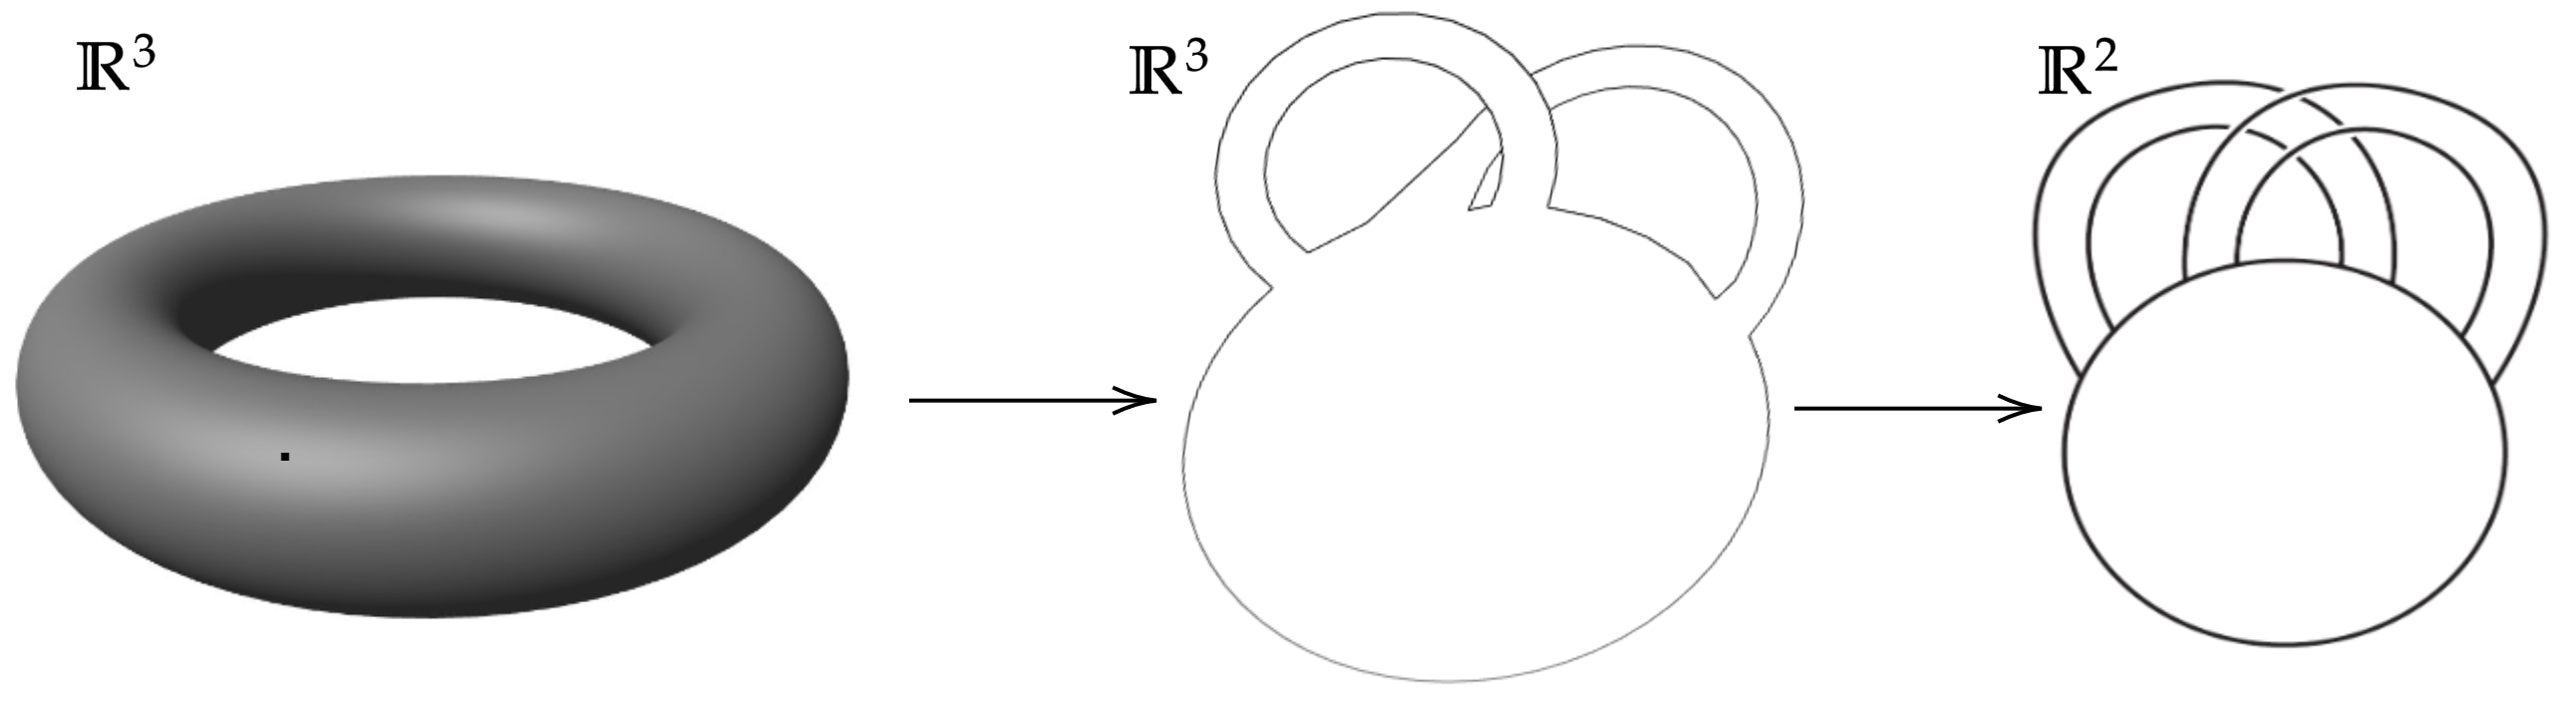
\includegraphics[width=0.8\textwidth]{toro_punteado}
  				\label{fig:toro_punteado}
			\end{figure}
			
			Sea $h:\mathbb{R}^2 \rightarrow S$ el embebimiento del enunciado, por el cual, haciendo ``pull-back'', la estructura diferenciable de $S$ induce una estructura diferenciable en $\mathbb{R}^2$, que denotaremos $E_1$. Por el mismo razonamiento pero para la inmersión $q$, $\mathbb{R}^2$ con la estructura $E_1$ induce una estructura diferenciable en $T'$ que llamaremos $E_2$.\\
			\\ Sabemos por el \textbf{Hecho 3} que existe un conjunto compacto en $T'_{E_2}$ cuyo complemento es difeomorfo a $S^1\times \mathbb{R}$ con su estructura diferenciable estándar, equivalentemente es difeomorfo a $D^2 - {(0,0)}$ como abierto de $\mathbb{R}^2$ con su estructura diferenciable estándar. Si vemos el disco punteado como un subconjunto del plano complejo $\mathbb{C}$, el $0$ se puede añadir de forma natural puesto que la estructura diferenciable usada hasta el momento es la usual en el cilindro (que induce la usual en $D^2$, en el plano complejo y en la esfera de Riemann). Esto nos permite extender la estructura diferenciable $E_2$ de $T'$ a $T$, la cual seguiremos llamando $E_2$.\\
			\\ Por el \textbf{Hecho 4} sabemos que toda estructura diferenciable del toro ($T \equiv S^1\times S^1$) es difeomorfa a la estándar. Por tanto, existe un difeomorfismo $g: T_{E_2} \rightarrow T$. Para poder utilizar el Teorema de Levantamiento de aplicaciones de la teoría de recubridores, necesitamos normalizar dicha función $g$:
						
			\begin{itemize}
				\item Aplicando rotaciones en el toro $T$ (lo vemos como $S^1\times S^1$) podemos hacer que $g$ lleve el $0$ en el $0$.
				\item Necesitamos que el homomorfismo $g_*$ sea la identidad a nivel de grupos fundamentales para que el difeomorfismo $g$ pueda ser levantado a un difeomorfismo $\widehat{g} : \mathbb{R}^2_{E_1} \rightarrow \mathbb{R}^2$ fijando el origen. Para ello basta con componer $g$ con el automorfismo lineal $L \in GL_2(\mathbb{Z})$ apropiado, es decir, aquel tal que al componerlo con $g_*$ queden fijos los dos generadores del grupo fundamental del toro topológico. La nueva $g$ sigue llevando el $0$ en el $0$ y $g_*$ es la identidad.\\
			\end{itemize}
			
			\begin{figure}[h]
  				\centering
  				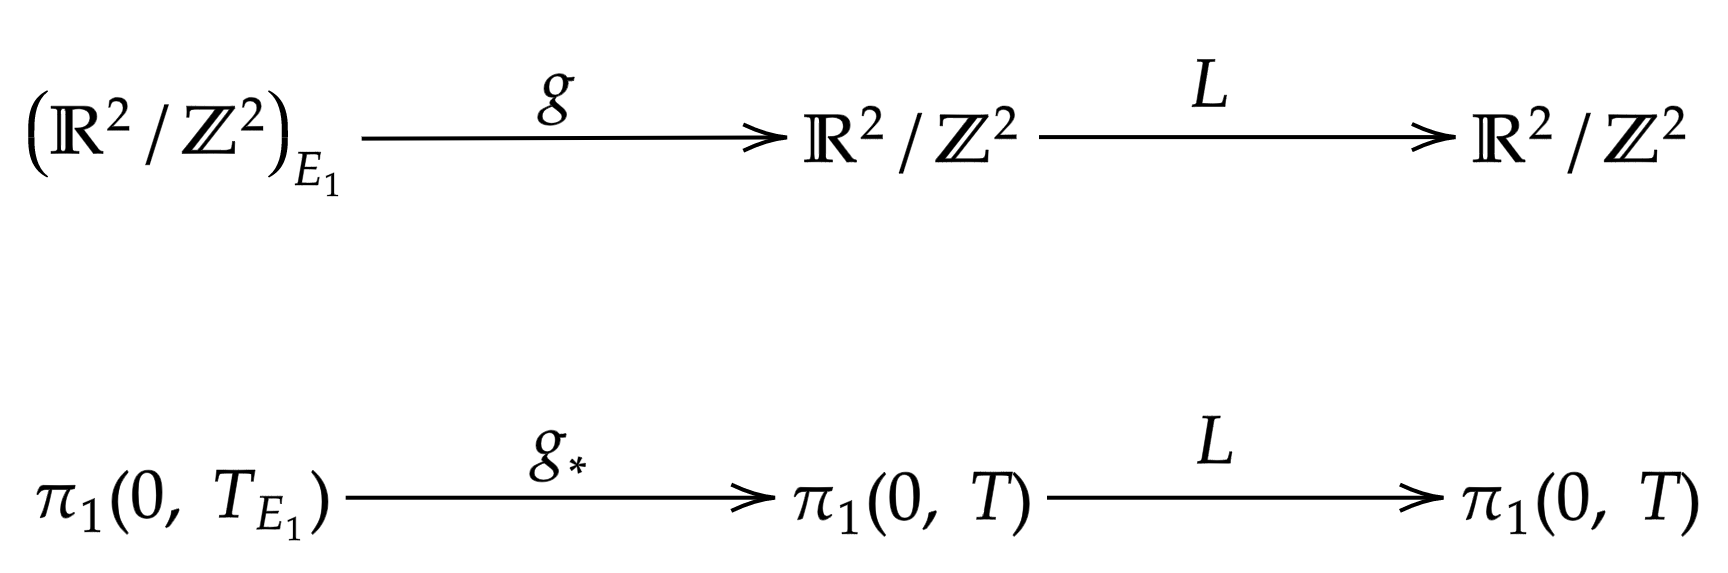
\includegraphics[width=0.5\textwidth]{grupos_fundamentales}
  				\label{fig:fundamental}
			\end{figure}
			 
			De esta forma construimos un difeomorfismo $\widehat{g}:\mathbb{R}^2_{E_1} \rightarrow \mathbb{R}^2$ como el levantamiento de $g$ fijando el origen, que de forma natural es doblemente periódico.\\
			
			\begin{figure}[h]
  				\centering
  				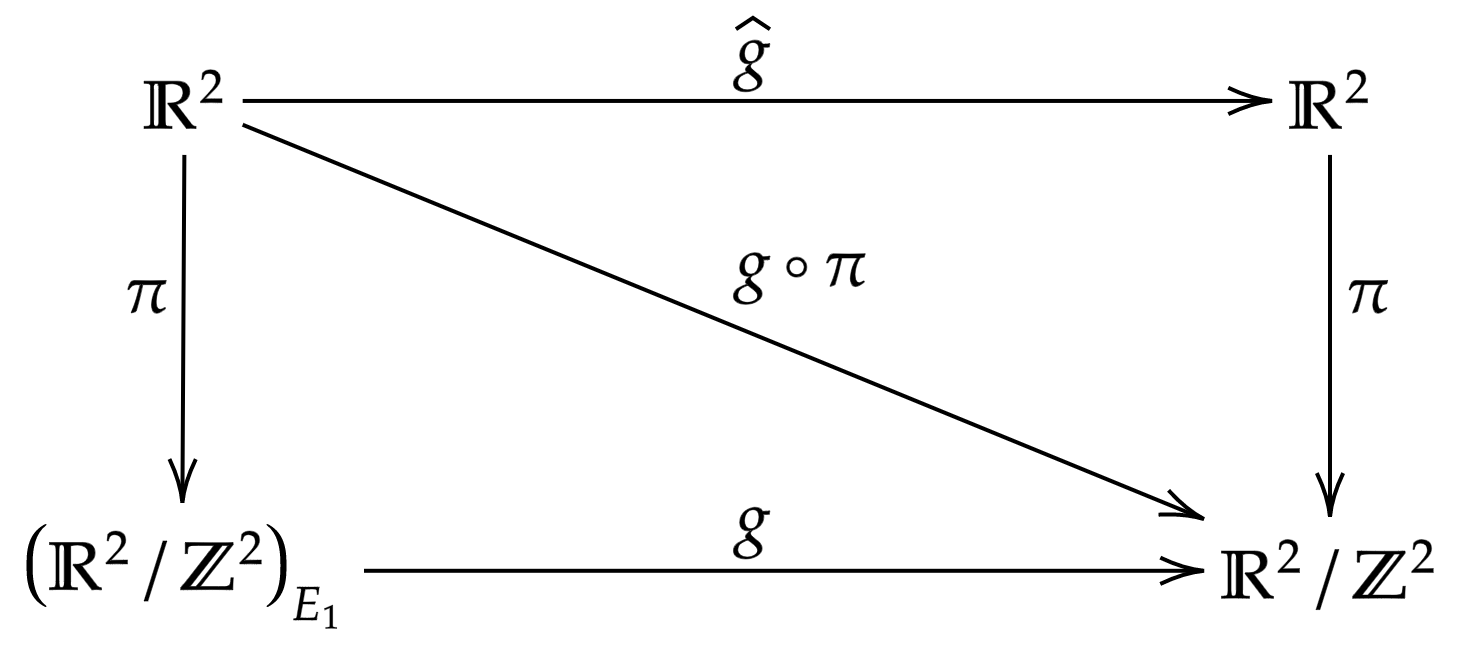
\includegraphics[width=0.5\textwidth]{levantamiento}
  				\label{fig:levantamiento}
			\end{figure}
			
			Identifiquemos $\R^2$ con el disco unidad $D^2$ de $\R^2$ vía un difeomorfismo radial (respecto de la estructura diferenciable estándar), que sea la identidad en un entorno del origen. A continuación traslademos vía ese difeomorfismo la estructura diferenciable $E_1$ de $\R^2$ al disco $D^2$, generando una estructura $E$ en el disco $D^2$, y análogamente la estructura diferenciable estándar de $\R^2$ que induce la estructura diferenciable estándar en $D^2$. Entonces, salvo estas identificaciones en el dominio y codominio de $\widehat{g}$, obtenemos $G:D^2_{E} \rightarrow D^2$ automorfismo diferenciable, que sigue siendo $\widehat{g}$ entorno al $0$ y tiende a ser la identidad en el borde (por la periodicidad $\|\widehat{g}(x) - x\|$ está acotado para todo $x$, y por consiguiente al tender $x$ a infinito las variaciones tienden a $0$ con la reparametrización, es decir, $G(x)$ tiende a $x$). Podemos extender $G$ a un homeomorfismo $G:\mathbb{R}^2_{E} \rightarrow \mathbb{R}^2$, siendo la identidad fuera del interior del disco.\\
			\\ Por el truco de Alexander, $G$ es isotópica a la identidad. Se puede obtener la isotopía $G_t$ variando el radio del disco de origen y destino ($G_t(x) = tG(\frac{x}{t})$ para $x \in D((0,0), t)$ y la identidad fuera del disco $D((0,0), t)$), por lo que $G_0$ es la identidad y $G_1=G$.\\
			\\ Definimos la isotopía que resuelva el problema como $h_t=h\circ G_t^{-1}$, teniendo que $h_0=h$ por ser $G_0$ la identidad. Además, $h_t$ se queda fija fuera del disco unidad ya que $G_t$ es la identidad en dicho conjunto. También tenemos que $h_t(0)=h(0)=0$ ya que para todo t, $G_t^{-1} = \widehat{g}^{-1}$ entorno al $0$ y $\widehat{g}(0)=0$. Finalmente, $h_1$ es diferenciable entorno al $0$ porque $G_1^{-1}=G^{-1} = \widehat{g}^{-1}$ entorno al $0$, que localmente es un difeomorfismo de la estructura usual de $\mathbb{R}^2$ en la inducida por $S$ mediante $h$, que habíamos denotado por $E_1$.
		\item La idea es, al igual que en el punto anterior, encontrar un automorfismo diferenciable del dominio de $h$ con diferentes estructuras diferenciables y restringirlo para que esté fijo donde lo solicite el enunciado.\\
			\\ Tenemos $h: D^1\times \mathbb{R} \rightarrow S$ embebimiento diferenciable en un entorno del borde del dominio. Dicho embebimiento induce una estructura diferenciable $E_1$ en $D^1\times \mathbb{R}$ que coincidirá con la estructura diferenciable estándar de $D^1\times \mathbb{R}$ entorno al borde ya que $h$ es diferenciable en el sentido usual ahí.\\
			\\ Por el \textbf{Hecho 5} tenemos que existe un difeomorfismo $g$ entre la estructura inducida $E_1$ y la estructura estándar de $D^1\times \mathbb{R}$ que es la identidad entorno al borde del conjunto. Tomamos el homeomorfismo $q: D^1\times \mathbb{R} \rightarrow (D^1\times D^1) - (0 \times \partial D^1)$ cuya acción se sugiere en la siguiente figura; en particular $q$ es la identidad en un entorno de $D^1 \times 0$.
			
			\begin{figure}[h]
  				\centering
  				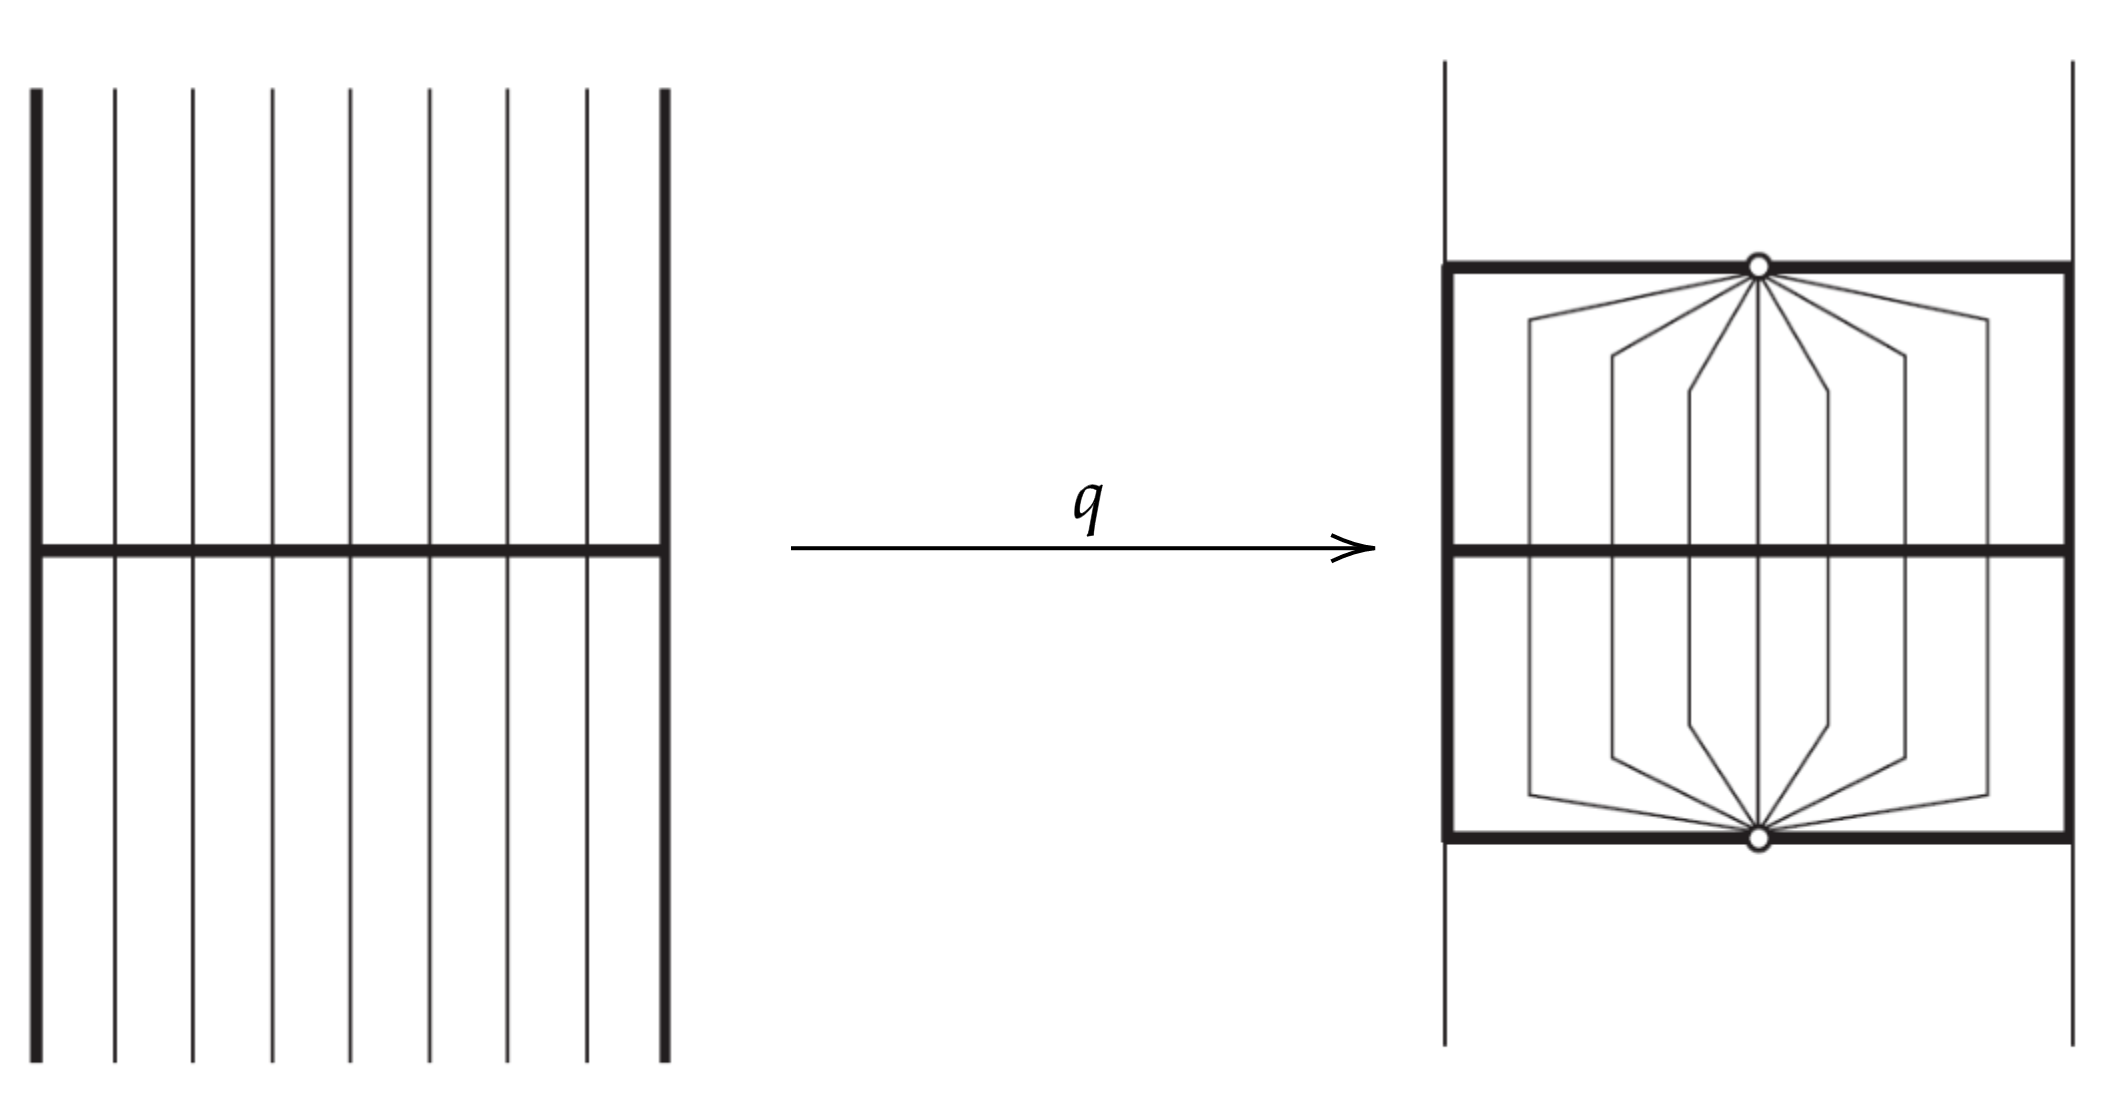
\includegraphics[width=0.5\textwidth]{embebimiento_q}
  				\label{fig:embebimiento_q}
			\end{figure}
			
			Como en el caso anterior trasladamos las correspondientes estructuras diferenciables vía $q$ y definimos $G:  ((D^1\times D^1) - (0 \times \partial D^1))_{E_1} \rightarrow (D^1\times D^1) - (0 \times \partial D^1)$ por $G = q \circ g \circ q^{-1}$, que como es la identidad entorno al borde del dominio, se puede extender a $G:\mathbb{R}^2_{E_1} \rightarrow \mathbb{R}^2$ como la identidad fuera de $D^1 \times D^1 - (0 \times \partial D^1)$. No hay problema en los dos puntos de $0 \times \partial D^1$ ya que por la definición de $q$ el difeomorfismo $G$ extiende dejándolos fijos.. Su comportamiento entorno a $D^1 \times 0$ es igual que el de $g$ ($q$ es la identidad) y es la identidad fuera de $D^1 \times D^1$ y entorno a $\partial D^1 \times \mathbb{R}$.\\
			
			\begin{figure}[h]
  				\centering
  				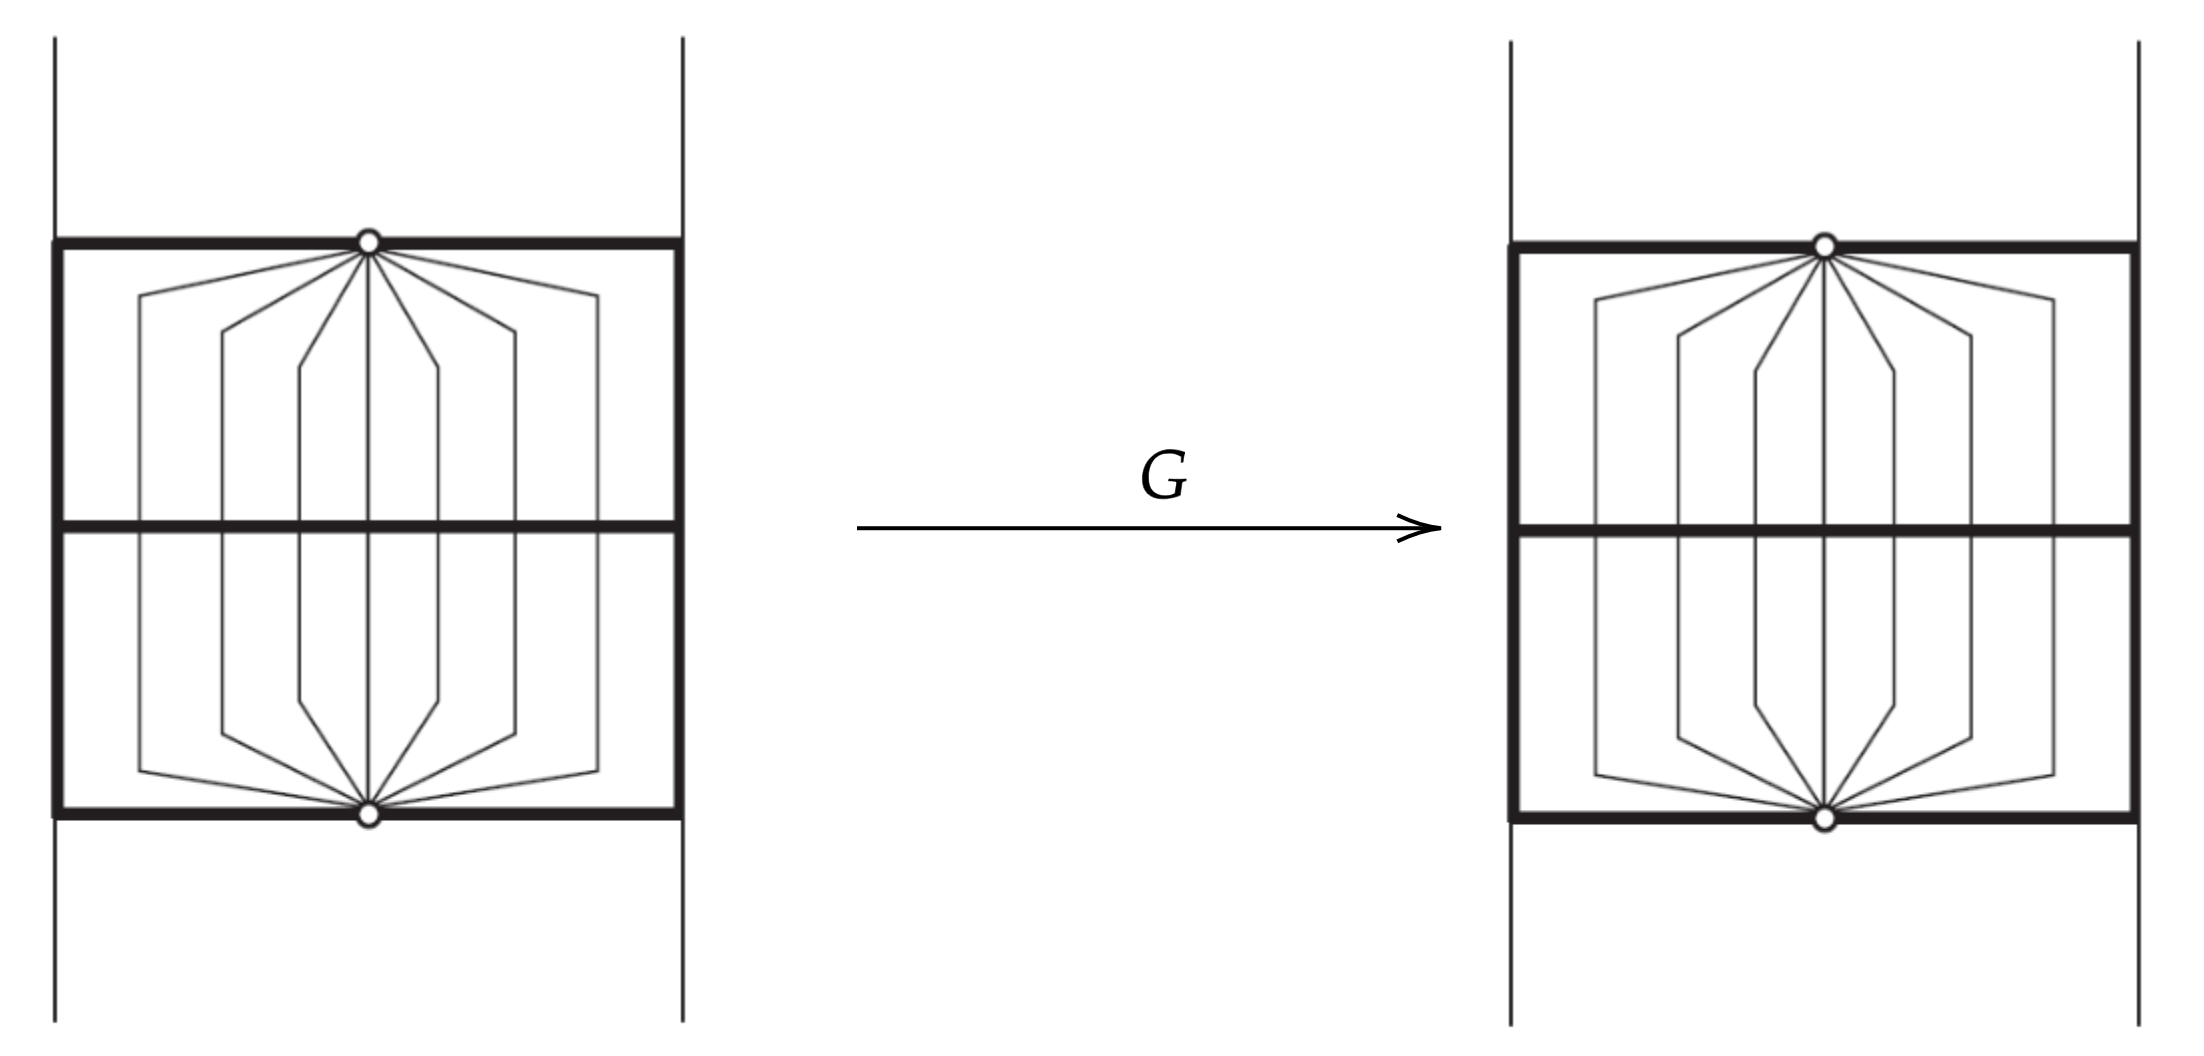
\includegraphics[width=0.5\textwidth]{g_inicial_extension}
  				\label{fig:g_inicial_extension}
			\end{figure}
			
			Podemos adaptar el truco de Alexander definiendo una isotopía $G_t$ de homemomorfismos en $\mathbb{R}^2$ rescalando el cuadrado $D^1 \times D^1$ al igual que en el apartado anterior hicimos con el disco, de forma que $G$ sea isotópica a la identidad en $\mathbb{R}^2$.\\
			\\ Finalmente basta con definir $h_t = h \circ G_t^{-1}$. Cumple claramente que $h_0 = h$, $h_1$ es diferenciable en un entorno de $D^1 \times 0$ y $h_t$ es la identidad en un entorno de $\partial D^1 \times \mathbb{R}$.
		\item Tenemos $h: D^2 \rightarrow S$ embebimiento que es diferenciable entorno al borde del dominio. Este embebimiento induce mediante ``pull-back'' la estructura diferenciable de $S$ a $D^2$ que coincide con la estructura diferenciable estándar de $D^2$ en un entorno del borde, ya que $h$ es diferenciable en dicha zona en el sentido usual.\\
			\\ Por el $\textbf{Hecho 6}$ existe un difeomorfismo $g$ entre $D^2$ con la estructura estándar y la inducida, que además es la identidad entorno al borde. Una adaptación del truco de Alexander al disco nos aporta la isotopía $g_t$ de homeomorfismos de $D^2$, donde $t$ va variando el tamaño de los discos de dominio e imagen de $g$ y extendiendo por la identidad, por lo que $g_0$ sería la identidad y $g_1 = g$. Tomando la isotopía $h_t = h \circ g_t$ tendríamos lo solicitado, ya que $h_0 = h$ y $h_1$ es igual que $h$ en un entorno del borde y es diferenciable en todo el disco.
	\end{enumerate}
	
\end{proof}


\begin{corolario}
	El primer apartado del teorema anterior sigue siendo cierto para un abierto $W$ de $\mathbb{R}^2$ en vez de para todo $\mathbb{R}^2$, con el objetivo de suavizarlo en un punto $p \in W$.
\end{corolario}

\begin{proof}
	Dado un punto $p \in W$, por ser un conjunto abierto existe una bola abierta $p \in B_p \subset W$. Tomamos $f: \R^2 \rightarrow B_p$ homeomorfismo que lleva el origen a $p$, cuya restricción a la bola abierta de radio $2$ centrada en el origen ($B((0,0), 2)=B_2$) es diferenciable. Tenemos que $f_{B_2} : B_2 \rightarrow f(B_2) \subset B_p$ es un difeomorfismo.\\
	\\Definimos $g=h \circ f: \R^2 \rightarrow S$ que es trivialmente continua e inyectiva. Como $f$ es un homeomorfismo y $h$ un embebimiento, la restricción de $g$ a su imagen es un homeomorfismo, y por tanto $g$ es un embebimiento.\\
	\\Aplicamos el primer apartado del teorema anterior a $g$, obteniendo la isotopía $g_t$, donde $g_1$ es diferenciable en un entorno del origen y queda fija fuera de un compacto que contiene al anterior. Además, por la demostración del teorema sabemos que dicho compacto está contenido en la bola abierta $B_2$, por lo que podemos construir la isotopía $h_t$ de la siguiente forma:
	\begin{itemize}
		\item $h_t(p)=(g_t \circ f_{f(B_2)}^{-1})(p)$ para todo $p \in f(B_2)$.
		\item $h_t(p)=h(p)$ para todo $p \in W - f(B_2)$.
	\end{itemize}
	Sabemos que pega bien debido a que $g_t$ deja fija a $g$ fuera de un compacto que contiene al origen y está contenido en $B_2$. De esta forma tendríamos una isotopía que deforma $h$ en una función que es diferenciable en un entorno del punto $p$ y queda fija fuera de un compacto que contiene al anterior, concluyendo así la prueba.
\end{proof}


\endinput
%------------------------------------------------------------------------------------
% FIN DEL CAPÍTULO. 
%------------------------------------------------------------------------------------


\endinput
%------------------------------------------------------------------------------------
% FIN DEL CAPÍTULO. 
%------------------------------------------------------------------------------------

% !TeX root = ../libro.tex
% !TeX encoding = utf8

\chapter{Resultados principales}

\section{Enunciados}
	\begin{teora}
		Toda variedad topológica 2-dimensional tiene una estructura diferenciable.
	\end{teora}

	\begin{teorb}
		Todo homeomorfismo entre variedades diferenciables 2-dimensionales es isotópico a un difeomorfismo.
	\end{teorb}
	
	Suponiendo ciertos los teoremas anteriores, es directa la obtención del siguiente resultado, ya que por A tenemos que toda variedad topológica 2-dimensional tiene una estructura diferenciable y por B sabemos que es única salvo difeomorfismos:
	
	\begin{corolario} (Teorema clásico de Munkres)
		Toda variedad topológica 2-dimensional tiene una única estructura diferenciable salvo difeomorfismos.
	\end{corolario}

\section{Demostración del Teorema A}

	\begin{teora}
		Toda variedad topológica tiene una estructura diferenciable.
	\end{teora}
	\begin{proof}[Demostración]
		Sea S una variedad topológica sin borde, podemos coger un sistema coordenado de cartas finito $\{(V_i, h_i)/ 1\leq i\leq N\}$. Vamos a construir por inducción una estuctura diferenciable en el conjunto $U_n = \cup_{i\leq n}h_i(\mathbb{R}^2)$, que por ser un sistema coordenado su límite debe de ser S, probando así el resultado. Cabe destacar que cada $U_i$ contiene a todos los anteriores. \\
		\\ La inducción empieza tomando una carta cualquiera del sistema, $U_1=V_1$ por ejemplo. Si se considera la variedad $U_1$ con el atlas $\{(h_1,U_1)\}$ entonces $h_1$ es diferenciable para ésta de forma trivial (se compone con la inversa y queda la identidad en $\mathbb{R}^2$).\\
		\\ Una vez arrancada la inducción, suponiendo cierto para el paso $n-1$ vamos a extender la diferenciabilidad de $U_{n-1}$ a $U_n$. Sea la carta $(V_n, h_n)$, tomamos entonces $W=h_n^{-1}(U_{n-1})=h_n^{-1}(U_{n-1}\cap h_n(V_n))$, que es un abierto de $\mathbb{R}^2$ por ser $h_n$ un homeomorfismo de $\mathbb{R}^2$ a $V_n$. \\
		\\ Tenemos $W\subset V_n$ abierto en $\mathbb{R}^2$, por el \textbf{Hecho 1} sabemos que existe una triangulación geométrica suya y que al ser abierto (no tiene borde) al ir acercándose al borde los triángulos tienden a ser puntos. Queremos aplicar el ``Teorema de alisamiento de asas'' en los vértices de los triángulos, seguidamente en los lados y finalmente en el interior de cada uno (aplicar los 3 apartados del teorema de forma consecutiva), pero para ello es necesario partir de un embebimiento de $\mathbb{R}^2$:
		\begin{enumerate}
			\item Para cada vértice $p$, elegimos una bola abierta lo suficientemente pequeña de forma que sus cierres no se corten (lo hacemos para todos los vértices de una vez), $B(p,\varepsilon _p)\subset W$ que es difeomorfo a $\mathbb{R}^2$ ($f_p:\mathbb{R}^2\rightarrow B$ difeomorfismo, con $f_p(0)=p$). Tomamos $g=h_n\circ f_p:\mathbb{R}^2\rightarrow h_n(W)$, que es un embebimiento por serlo $h_n|_B:B\rightarrow h_n(W)$ y $f_p$ (la composición de embebimientos es un embebimiento). \\
			\\ Aplicamos el apartado 1 del Teorema de alisamiento de asas y obtenemos una $\widehat{g}$ isotópica a la primera, que es diferenciable en $O_p$ (entorno abierto del origen, con $0=f_p^{-1}(p)$) y además queda fija fuera de otro entorno un poco mayor $O_p'\supset O_p$, con $\overline{f_p(O_p)}\subset B $. Si tomamos la función a trozos $\widehat{h}_n|_{B}=\widehat{g}\circ f_p^{-1}$ y $\widehat{h}_n|_{W-B}=h_n$, está bien definida porque en $B-f_p(O_p)$ al aplicar $f_p^{-1}$ nos lleva a $\mathbb{R}^2-O_p$, que es donde $\widehat{g}=g$, es decir: \\
			\begin{center}
				$\widehat{h}_n|_{B-f_p(O_p)}=\widehat{g}\circ(f_p^{-1}|_{B-f_p(O_p)})=g\circ(f_p^{-1}|_{B-f_p(O_p)})=h_n|_{B-f_p(O_p)}$\\
			\end{center}
			por lo que la función a trozos está bien definida, es diferenciable entorno a $p$ y no se altera fuera de $B$. \\
			\\ Éste paso se puede realizar de forma simultánea para todos los vértices, obteniendo así una $\widehat{h}_n$ que es diferenciable entorno a todos los vértices y se mantiene $h_n$ fuera de un entorno de cada vértice, algo mayor que el anterior (entornos con cierres disjuntos). Es por ello que para no cargar demasiado la notación se llamará a esa nueva función $h_n$.
			\item Tenemos un $h_n$ que es diferenciable entorno a los vértices de los triángulos y queremos usar el apartado 2 del Teorema de alisamiento de asas para extender la diferenciabilidad a un entorno tubular de los lados de los triángulos. Para ello, vemos que en cada lado, junto con los entornos de los vertices, podemos incluir un rectángulo abierto (conjunto abierto de $W$) que contenga a todo el segmento y cuyos segmentos laterales del rectángulo estén contenidos en ambas bolas. Este conjunto es difeomorfo a $\mathbb{R}^2$ y aplicando previamente dicho difeomorfismo cumplimos las hipótesis deseadas.\\
			\\ Al proseguir de forma semejante al apartado anterior, conseguimos una función $h_n$ que es diferenciable en un entorno del conjunto de todos los lados, quedando fija fuera de un entorno algo más grande.
			\item Buscamos finalmente una curva dentro del``esqueleto'' de entornos de los lados de los triángulos que junto con su componente interior sea difeomorfa a la bola cerrada unidad, para aplicar el 3$^{er}$ apartado del Teorema de alisamiento de asas y así obtener una $h_n$ diferenciable en todo $W$.\\
			\\ La curva buscada debe ser diferenciable, cerrada y simple, para así decir que es una curva de Jordan y aplicar el Teorema de la curva de Jordan. Como consecuencia, sabemos que su componente interior es difeomorfa a la bola unidad de $\mathbb{R}^2$. Podemos reducir el problema a buscar dicha curva para el entorno tubular de un triángulo equilátero, ya que es difeomorfo al de un triángulo cualquiera. Además, podemos seguir simplificándolo, aportando únicamente una curva no cerrada cuyos extremos se puedan pegar consecutivamente, siendo infinitamente derivable en los puntos donde se unen.\\
			\\ Haciendo uso de una función meseta $f$ que vale $0$ en $\mathbb{R}^-$ y $1$ a partir de $\epsilon > 0$, si tomamos $g(x)=tg(\frac{\pi}{3})xf(x)$ en el intervalo $[-1,\epsilon]$, tenemos que $g(-1)=0$ y $g(\epsilon)=tg(\frac{\pi}{3})\epsilon$  al igual que sus derivadas, por lo que si vamos alternando $g(x)$ y $g(-x)$ mediante rotaciones y traslaciones, tendremos una curva $\alpha$ diferenciable (suavización del triángulo equilátero). \\
			%\newpage
			\begin{figure}[h]
  				\centering
  				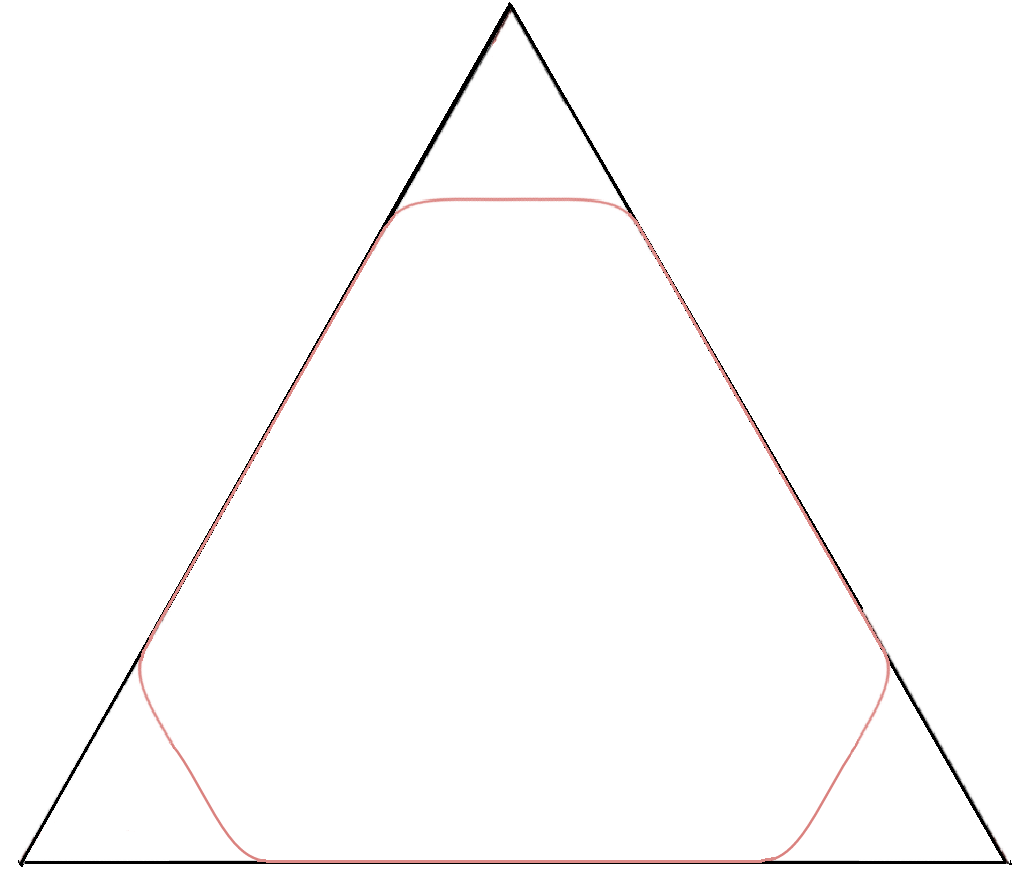
\includegraphics[width=0.5\textwidth]{triangulo_suavizado}
  				\caption{Curva de Jordan cercana al triángulo}
  				\label{fig:triangulo_suavizado}
			\end{figure}
			\\ Se puede observar que es válido $\forall \epsilon > 0$ y que al hacer tender $\epsilon$ a $0$, la curva será el propio triángulo equilátero. Es por ello que podemos tomar el $\epsilon$ lo suficientemente pequeño como para que la curva $\alpha$ quepa en el entorno tubular y siga siendo una curva de Jordan. \\
			\\ Ya tenemos un difeomorfismo entre la bola unidad y la componente interior de cada uno de los triángulos, que contienen un abierto conexo en el cual la función no es todavía diferenciable. Estamos en las condiciones del punto 3 del Teorema de alisamiento de asas, así que procediendo de igual forma que en los apartados anteriores obtenemos una $h_n$ totalmente diferenciable en $W$.
		\end{enumerate}
		
		Cabe destacar que en el borde de $W$ la aplicación se queda intacta, ya queen todo momento se está trabajando en el interior de $W$ (es abierto) y en todo paso de la "suavización" de $h_n$ siempre se deja inalterado el espacio complemento de un entorno mayor al aquel donde se obtiene la diferenciabilidad. Es por ello que se puede extender el $h_n$ obtenido a todo $\mathbb{R}^2$ junto con el original, porque está bien definido, quedando intacta en $\mathbb{R}^2-W$. 
	\end{proof}

\section{Demostración del Teorema B}
	\begin{teorb}
		Todo homeomorfismo entre variedades diferenciables 2-dimensionales es isotópico a un difeomorfismo.
	\end{teorb}
	\begin{proof}[Demostración]
		Sea $f: S \rightarrow S'$ homeomorfismo entre variedades diferenciales 2-dimensionales, se pueden dar 2 casos:
		\begin{enumerate}
			\item $\partial S = \phi$, por lo que podemos utilizar el \textbf{Hecho 2}, que nos aporta una triangulación diferenciable. Si utilizamos el mismo sistema coordenado que para la demostración del Teorema A, al aplicar $h_i^{-1}$ a dicha triangulación diferenciable, por definición tenemos una triangulación clásica en $\mathbb{R}^2$. Si componemos $f$ con $h_i$ ($g=f\circ h_i$), tenemos un embebimiento $g: \mathbb{R}^2 \rightarrow S'$.\\
			\\ Aplicando los apartados del Teorema de alisamiento de asas conseguimos un embebimiento diferenciable $\widehat{g}$ isotópico a $g$, y tomando $\widehat{f}=\widehat{g}\circ h_i^{-1}$ tenemos un homeomorfismo diferenciable isotópico a $g\circ h_i^{-1}=f$. De forma simétrica, aplicándolo a $\widehat{f}^{-1}$, obtenemos que $f$ es isotópico a un difeomorfismo. 
			\item $\partial S \neq \phi$, podemos considerar un collar diferenciable de $\partial S$ en $S$ e isotopar f a a un homeomorfismo diferenciable cerca del borde, dentro de ese conjunto, independientemente del difeomorfismo elegido para el collar diferenciable. Dicha isotopía se obtendrá utilizando el Teorema de alisamiento de asas, tal y como se ha hecho en el apartado anterior. La isotopía dejará fija a $f$ fuera del collar diferenciable. Lo hacemos de igual forma para la inversa, obteniendo una isotopía que deja fija a $f^{-1}$ fuera de un collar diferenciable del borde de $S'$, siendo diferenciable en otro collar diferenciable contenido en el anterior.\\
			\\ Ahora partimos de un homeomorfismo diferenciable en el borde de $S$, aplicando lo utilizado en el apartado anterior podemos obtener una isotopía a $\widehat{f}$, que es un difeomorfismo de $S$ a $S'$,ya que se puede tomar una triangulación en los interiores de las superficies (entendemos por interior a la superficie menos su borde). Aplicamos los mismos pasos para la inversa de $\widehat{f}$, obteniendo así que $f$ es isotópico a un difeomorfismo en todo $S$.
		\end{enumerate}
	\end{proof}
\endinput
%------------------------------------------------------------------------------------
% FIN DEL CAPÍTULO. 
%------------------------------------------------------------------------------------


\cleardoublepage
\setpartpreamble[c][0.75\linewidth]{%
	\bigskip % Deja un espacio vertical en la parte superior
  Si el trabajo se divide en diferentes partes es posible incluir al inicio de cada una de ellas un breve resumen que indique el contenido de la misma. Esto es opcional.
}\part{Visualización de superficies}

% !TeX root = ../libro.tex
% !TeX encoding = utf8

\chapter{Estudio de la teselación}

En este capítulo se describe el estudio realizado para teselar de manera eficiente un triángulo. Esta técnica se implementará en shaders, para poder ejecutarlo directamente en la GPU, que ofrece mayor rendimiento que la CPU para dicho problema. En un principio se iba a realizar en un Geometry Shader pero más tarde se observó que era más acertado el uso de un Tessellation Shader. \\
\\ Cabe destacar antes que la idea inicial era desarrollar un algoritmo de división recursiva de los triángulos, el cuál se detiene en el nivel en el que se cree que representa correctamente a la porción de superficie. Sin embargo, el lenguaje Glsl no permite realizar llamadas recursivas, por lo que era necesario buscar alternativas.

\section{Geometry shader}
	La ventaja de este tipo de shader es que es muy flexible a la hora de generar nuevas primitivas, ya que permite añadir primitivas totalmente disconexas.\\
	\\ En primer lugar opté por describir de forma explícita un cierto número de niveles de la función recursiva deseada, $3$ niveles concretamente. Los resultados eran aceptables pero se podía exceder el límite de vértices, quedando así una superficie incompleta. Además, el tiempo de compilación crecía de forma exponencial a medida que se añadían más niveles (para $2$ niveles era de $10$-$15$s y para $3$ no concluía).\\
	\\ Puesto que este método era costoso temporalmente y tenía muchas limitaciones, decidí implementar un algoritmo similar pero en un bucle, cuyo esquema es el siguiente:
	\begin{enumerate}
		\item Dado un lado, dividirlo en tantos segmentos como sea necesario, atendiendo a una cierta medida. Dicha medida sólo depende de las características del lado, para que el pegado sea el correcto con los triángulos adyacentes.
		\item Se realiza una división hacia el baricentro, de forma similar al punto anterior.
		\item Con los vértices de los dos puntos anteriores se genera una malla, es decir, para cada lado, se genera otro lado paralelo para cada subdivisión hacia el baricentro, manteniendo proporcionalmente las subdivisiones del lado original.
		\item Se genera una tira de triángulos cuyos vértices sean los de la malla anterior.
	\end{enumerate}
	
	Con este método los problemas anteriores se solventan en gran medida, pero dicho algoritmo es semejante al del Tessellation shader, por lo que era natural estudiar el funcionamiento en tal shader.\\
	\\ Finalmente, los inconvenientes observados han sido los siguientes:
	\begin{itemize}
		\item El número de vértices de salida está limitado por una constante predefinida, con valor GL$\_$MAX$\_$GEOMETRY$\_$OUTPUT$\_$VERTICES=$256$ (depende del hardware), es decir, como mucho se puede devolver una tira de $254$ triángulos, independientemente del tamaño del triángulo original.
		\item El shader tarda en compilarse de media entre $3$ y $5$ segundos.
	\end{itemize}
	
\section{Tessellation shader}

	Este shader tiene un pequeño problema y es que la subdivisión está predefinida (equal, fractional$\_$odd o fractional$\_$even spacing), por lo que los vértices generados en la fase de control del Tessellation shader tienen un esquema fijo, para un número de subdivisiones dado. No es un gran inconveniente puesto que en la fase de evaluación se pueden variar libremente dichos vértices, siempre que se haga con cuidado (en esta fase los vértices se generan mediante coordenadas baricéntricas). \\
	\\ Las ventajas con respecto al Geometry shader son las siguientes:
	\begin{itemize}
		\item El shader tarda en compilarse de media menos de $1s$.
		\item El número de vértices de salida no está tan limitado (GL$\_$MAX$\_$PATCH$\_$VERTICES$=36477$ frente a $256$).
		\item Está pensado para realizar directamente el algoritmo de teselación, por lo que no hay que implementarlo.
	\end{itemize}
	
	Al tener implementado el algoritmo de teselación, el estudio se reduce a encontrar una medida que nos indique cómo de buena es la representación de la superficie. Como la teselación se indica por cada lado (outer tessellation factor) y en el interior (inner tessellation), para cada tipo de medida hay que proporcionar una adicional para los lados, para que la teselación sólo dependa de lo que sucede en ellos y de esta forma pegue correctamente con el triángulo adyacente.
	
	\subsection{Medida basada en el volumen}
	
	Consiste en estimar el volumen de la diferencia entre el poliedro generado y la superficie original a nivel local. Esta medida está asociada al primer concepto de superficie bien representada:
	\begin{definicion}[Superficie bien representada 1]
		Dada una superficie $S$ y un politopo $P$ que la aproxima, se dice que la representa con una precisión de $\epsilon > 0$ si el volumen contenido entre ambos es menor que $\epsilon$.
	\end{definicion}
	La medida equivalente para los lados es el área de la sección cuya base es el lado del triángulo y el borde restante es la curva original a aproximar con dicho lado.\\ 
	\begin{figure}[h]
  		\centering
  		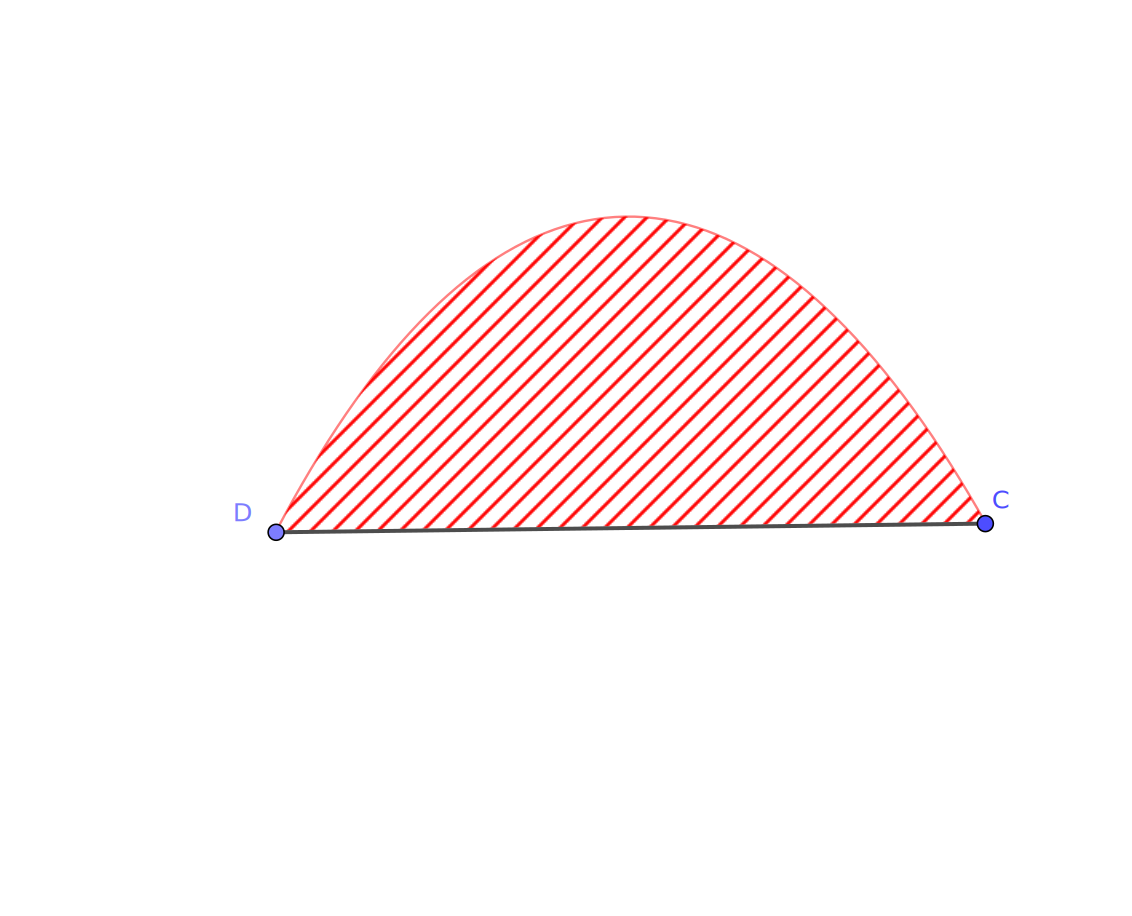
\includegraphics[width=0.5\textwidth]{seccion_area}
  		\caption{Medida en un lado $DC$}
  		\label{fig:seccion_area}
	\end{figure}
	\\ Sin embargo, para las superficies no compactas esta definición puede no permitir la existencia de un $P$ que la aproxime con una precisión finita.\\
	\\ Además, aparece el problema de la no detección de picos, debido a que al estudiar el volumen, si la altura es grande y la base lo suficientemente pequeña se puede dar el caso de que el volumen quede por debajo de la precisión $\epsilon$ y no tesele, aun existiendo dicho pico.
	\newpage
	\begin{figure}[h]
  		\centering
  		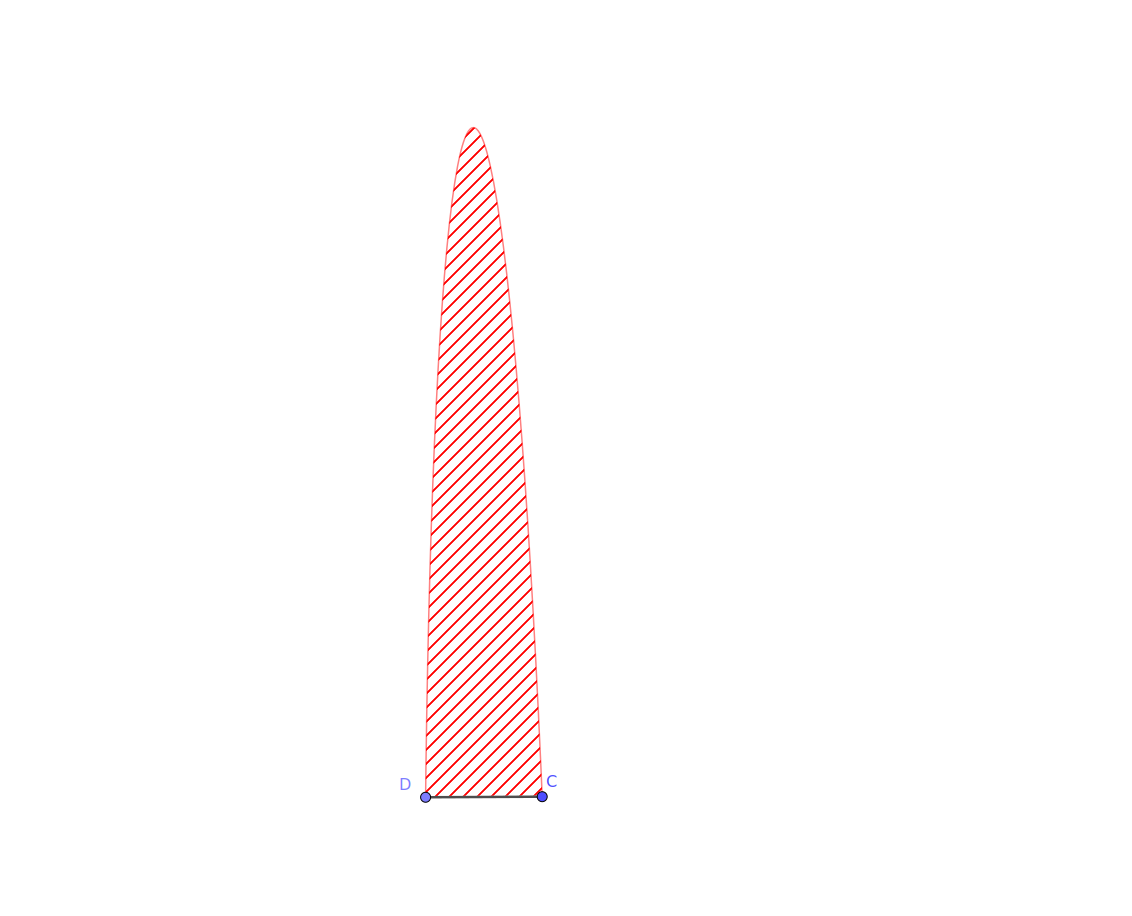
\includegraphics[width=0.6\textwidth]{pico_volumen}
  		\caption{Pico no teselado}
  		\label{fig:pico_volumen}
	\end{figure}
	
	\subsection{Medida basada en el área}
	
	Consiste en estimar el área de la superficie original localmente. Esta medida está asociada al segundo concepto de superficie bien representada:
	\begin{definicion}[Superficie bien representada 2]
		Dada una superficie $S$ y un politopo $P$ que la aproxima, se dice que la representa con una precisión de $\epsilon > 0$ si el ratio de área $r=\frac{A(S)} {A(P)}$ cumple que $r-1 < \epsilon$ (siempre se tiene que $r\geq 1$).
	\end{definicion}
	
	La medida equivalente para los lados es $r=\frac{L(\alpha)} {L(l)}$ donde $L$ es la longitud, $l$ el lado del triángulo y $\alpha$ la curva a estimar.\\
	\\Es una buena alternativa para poder detectar dichos picos, ya que cuando hay uno o varios picos mal aproximados el área original entorno al pico es mucho mayor que la de la superficie generada (el ratio es grande). Además, de esta forma estamos evitando la aparición del problema del farolillo de Schwarz (--CITAR--) debido a que buscamos estimar con una cierta precisión el área original.
	
	\subsection{Medida basada en la curvatura}
	Consiste en estimar la curvatura de Gauss por área. Esta medida está asociada al tercer concepto de superficie bien representada:
	\begin{definicion}[Superficie bien representada 3]
		Dada una superficie $S$ y un politopo $P$ que la aproxima, se dice que la representa con una precisión de $\epsilon > 0$ si para todo triángulo $T$ del politopo se cumple que $K_T A(T) < \epsilon$, donde $K_T$ es el máximo valor de la curvatura de Gauss en valor absoluto en $T$.
	\end{definicion}
	
	La medida equivalente para los lados es $K_l L$ donde $L$ es la longitud y $l$ el lado del triángulo.\\
	\\Si utilizamos como medida sólo la curvatura, que no depende de la parametrización de la superficie, teselaríamos de igual forma en un triángulo grande $T_1$ y en uno pequeño $T_2$ si $K_{T_1}=K_{T_2}$, obteniendo resultados distintos. Esto se debe a que la parametrización elegida deforma la malla inicial cambiando la densidad de triángulos. Un claro ejemplo es la reducción del tamaño de los triángulos a medida que nos acercamos a los polos en una esfera con la parametrización usual.\\
	\\Para evitarlo, multiplicamos por el área del triángulo, así que para el caso anterior el triángulo $T_1$ tendría un valor de dicha medida mayor que el triángulo $T_2$, por lo que sería necesario teselar más.\\
	\\Puesto que la escena es dinámica y es posible mover el punto de visión, se puede utilizar el área relativa al ``ojo'' en vez del área real, es decir, variar la teselación necesaria según la distancia del ojo a la superficie. Esto permite que a medida que nos acerquemos a la superficie, la teselación aumente, funcionando de manera similar a un gráfico vectorial escalable (SVG), pero en $\R^3$.
	
	
\section{Mejora del teselado}
	En esta sección vamos a estudiar cómo mejorar el proceso de teselado para mostrar buenos resultados sin tener un gran impacto en el rendimiento.
	\subsection{Teselado de bordes}
	\subsection{Mejora de rendimiento general}
		Hablar del no teselado fuera del view-frustum
	\subsection{Mejora de rendimiento específica}
		Hablar del no teselado en zonas ocultas y sin iluminación
	

\endinput
%------------------------------------------------------------------------------------
% FIN DEL CAPÍTULO. 
%------------------------------------------------------------------------------------



% --------------------------------------------------------------------
% BACKMATTER
% --------------------------------------------------------------------
\backmatter % desactiva la numeración de capítulos sin resetear la numeración de las páginas.

% !TeX root = ../libro.tex
% !TeX encoding = utf8

\chapter{Planificación y presupuesto}

\begin{center}
\begin{tabular}{ | p{0.5cm} | p{2.5cm} | p{5cm} | p{5cm} | }
\hline
\multicolumn{4}{ | c | } {Planificación temporal en fases}\\
\hline
\multicolumn{1}{ | c | } {Nº} & \multicolumn{1}{ | c | } {Nombre} & \multicolumn{2}{ | c | } {Tareas}\\
\hline
$1$ & Inicial & \multicolumn{2}{ | p{10cm} | } {- Estudio inicial del problema}\\
\hline
$2$ & Implementación básica & Procesador: & Visualizador:\\
 & & - Definición del lenguaje (BNF) & - Toma de contacto con OpenGL, el lenguaje GLSL e ImGui.\\
 & & - Implementar primera versión del procesador a partir del código de la asignatura Procesadores de Lenguajes, que sólo detecta errores. & - Construir un programa de visualización a partir de código base, haciendo uso de los shaders básicos. La normal será la del triángulo.\\
 & & - Complementar el procesador para traducir a código GLSL (generación de árbol sintáctico), para usarlo en el vertex shader. & \\
\hline
$3$ & Primera conexión & \multicolumn{2}{ | p{10cm} | } {- Conectar apropiadamente los programas, para visualizar la superficie definida con la parametrización.} \\
 & & \multicolumn{2}{ | p{10cm} | } {- Estudiar el correcto funcionamiento de ambas aplicaciones hasta ahora. Corregir en caso de ser necesario.} \\
 & & \multicolumn{2}{ | p{10cm} | } {} \\
\hline
\end{tabular}
\end{center}

- Implementación media.
9.- Implementar los algoritmos que calculan los árboles de las derivadas parciales de las expresiones. Añadir seguidamente la generación de funciones típicas, como la normal, el área diferencial y la curvatura de Gauss.
10.- Utilizar la función normal en los puntos, en vez de las normales de los triángulos. Además, mostrar la normal como un segmento de color distinto al de la superficie.
11.- Mostrar mediante colores el valor del área diferencial y de la curvatura de Gauss en cada punto.
12.- Estudiar el correcto funcionamiento de ambas aplicaciones hasta ahora. Corregir en caso de ser necesario.

- Implementación avanzada.
13.- Implementar la teselación uniforme mediante el uso del geometry shader.
14.- Completar con una gran variedad de ejemplos.
15.- Estudiar el correcto funcionamiento del teselado.

- Estudio de la mejor medida.
16.- Elegir ciertas estadísticas del renderizado para comprobar si los resultados son buenos.
17.- Estudiar varias medidas para controlar el nivel de teselado.

- Estética
18.- Completar la interfaz del usuario.

- Revisión
19.- Estudiar el correcto funcionamiento de ambas aplicaciones hasta ahora. Corregir en caso de ser necesario.

\endinput
%------------------------------------------------------------------------------------
% FIN DEL CAPÍTULO. 
%------------------------------------------------------------------------------------

\input{capitulos/analisis_diseño}
% !TeX root = ../libro.tex
% !TeX encoding = utf8

\chapter{Implementación y pruebas}

\section*{Tipo de shader para el teselado}
En esta sección se justificará el uso del tesellation shader para el estudio del teselado de una superficie.
 
\subsection*{Geometry shader}
	La ventaja de este tipo de shader es que es muy flexible a la hora de generar nuevas primitivas, ya que permite añadir primitivas totalmente disconexas.\\
	\\ En primer lugar opté por describir de forma explícita un cierto número de niveles de la función recursiva deseada, $3$ niveles concretamente. Los resultados eran aceptables pero se podía exceder el límite de vértices, quedando así una superficie incompleta. Además, el tiempo de compilación crecía de forma exponencial a medida que se añadían más niveles (para $2$ niveles era de $10$-$15$s y para $3$ no concluía).\\
	\\ Puesto que este método era costoso temporalmente y tenía muchas limitaciones, decidí implementar un algoritmo similar pero en un bucle, cuyo esquema es el siguiente:
	\begin{enumerate}
		\item Dado un lado, dividirlo en tantos segmentos como sea necesario, atendiendo a una cierta medida. Dicha medida sólo depende de las características del lado, para que el pegado sea el correcto con los triángulos adyacentes.
		\item Se realiza una división hacia el baricentro, de forma similar al punto anterior.
		\item Con los vértices de los dos puntos anteriores se genera una malla, es decir, para cada lado, se genera otro lado paralelo para cada subdivisión hacia el baricentro, manteniendo proporcionalmente las subdivisiones del lado original.
		\item Se genera una tira de triángulos cuyos vértices sean los de la malla anterior.
	\end{enumerate}
	
	Con este método los problemas anteriores se solventan en gran medida, pero dicho algoritmo es semejante al del Tessellation shader, por lo que era natural estudiar el funcionamiento en tal shader.\\
	\\ Finalmente, los inconvenientes observados han sido los siguientes:
	\begin{itemize}
		\item El número de vértices de salida está limitado por una constante predefinida, con valor GL$\_$MAX$\_$GEOMETRY$\_$OUTPUT$\_$VERTICES=$256$ (depende del hardware), es decir, como mucho se puede devolver una tira de $254$ triángulos, independientemente del tamaño del triángulo original.
		\item El shader tarda en compilarse de media entre $3$ y $5$ segundos.
	\end{itemize}
	
\subsection*{Tessellation shader}

	Este shader tiene un pequeño problema y es que la subdivisión está predefinida (equal, fractional$\_$odd o fractional$\_$even spacing), por lo que los vértices generados en la fase de control del Tessellation shader tienen un esquema fijo, para un número de subdivisiones dado. No es un gran inconveniente puesto que en la fase de evaluación se pueden variar libremente dichos vértices, siempre que se haga con cuidado (en esta fase los vértices se generan mediante coordenadas baricéntricas). \\
	\\Además, la versión de OpenGL necesaria es superior al del Geometry shader ($4.0$ frente a $3.2$).
	\\ Las ventajas con respecto al Geometry shader son las siguientes:
	\begin{itemize}
		\item El shader tarda en compilarse de media menos de $1s$.
		\item El número de vértices de salida no está tan limitado (GL$\_$MAX$\_$PATCH$\_$VERTICES$=36477$ frente a $256$).
		\item Está pensado para realizar directamente el algoritmo de teselación, por lo que no hay que implementarlo.
	\end{itemize}
	
	Al tener implementado el algoritmo de teselación, el estudio se reduce a encontrar una medida que nos indique cómo de buena es la representación de la superficie. Como la teselación de un triángulo se indica por cada lado (outer tessellation factor) y en el interior (inner tessellation), para cada tipo de medida hay que proporcionar una adicional para los lados, para que la teselación sólo dependa de lo que sucede en ellos y de esta forma pegue correctamente con el triángulo adyacente.

\section*{Optimización del código GLSL}
	Puesto que queremos que el programa renderice la escena en tiempo real, es necesario simplificar todo lo posible el código de los shaders, sobre todo del fragment shader (se va a ejecutar para cada vértice generado en el teselado). Para ello se han tenido en cuenta los siguientes hechos (FUENTE GLSL OPTIMIZATIONS):
	\begin{itemize}
		\item Evitar el uso de saltos condicionales y de bucles. En caso de ser necesario algún bucle, usar los de la forma ``for(int i=$0$; i<n; i++)'' con $n$ entero constante, para permitir el desenrollado del bucle por el compilador.
		\item Utilizar ``Swizzle'' en vez de asignar vectores componente a componente.
		\item Utilizar ``MAD'', es decir, usar siempre que sea posible la multiplicación por el inverso en vez de la división (para aquellos valores ``uniform'' o constantes) y desarrollar las expresiones como una sumatoria de productos. Por ejemplo, utilizar $a*0.5 + b*0.5$ en vez de $(a+b)/2$.
		\item Utilizar ``dot'' para agrupar varias expresiones en 1. De igual forma utilizar todo el cálculo vectorial y matricial posible para resumir las operaciones.
		\item Si una expresión es común para un mismo frame, calcularlo en la CPU y asignarlo como otro ``uniform'' para quitarle carga a la GPU, ya que se ejecutaría para cada primitiva o vértice (dependiendo de en qué shader se realize el cálculo).
	\end{itemize}
	
	Es cierto que el compilador ya realiza de manera automática algunas de estas optimizaciones, pero su puesta en práctica reduce ligeramente el tiempo de compilación.

\section*{Procesador}
La implementación del ``procesador'' nos se ha realizado desde cero, se ha partido de una implementación parcial que se aportaba en la asignatura de Procesadores de lenguajes. Dicha implementación, tras ser adaptada, sólo realizaba la traducción directa del código de entrada, junto con la comprobación de errores (léxicos, sintácticos y semánticos). La parte restante corresponde con la generación del árbol de expresión y calcular los árboles derivados, además de adecuar la salida correctamente para que se pueda utilizar como parte de un shader.

\section*{Visualizador}
En un principio se propuso utilizar como código de partida el proporcionado en la asignatura de Informática Gráfica, pero se observó que tenía muchas funcionalidades que no se llegarían a utilizar y cuya adaptación requeriría más tiempo. Por ello se decidió empezar de cero, pero utilizando como ``esqueleto'' un código de ejemplo de la referencia LearnOpenGL \cite{LearnOGL}, que aportaban simplemente la visualización de un objeto en una escena $3$D con una fuente de luz y una cámara sencilla.

\section*{Interfaz}
Para la implementación de la interfaz se ha utilizado la librería de código libre ``Dear ImGui'' \cite{DearImGui}, junto los complementos ``ImGui Quat'' \cite{LVector} para visualizar el vector de luz y modificarlo, e ``ImGui Dialog'' \cite{Dialog} para mostrar un diálogo con un explorador de archivo y así poder seleccionar la parametrización deseada.

\section*{Generación de informes}

	Para medir el rendimiento de la aplicación se han medido los fotogramas generados por segundo y las primitivas que hay presentes en la escena, incluyendo las que son producto del teselado.\\
\\La medición del nº de primitivas se ha realizado mediante el uso de la estructura "query" de OpenGL, la cual se actualiza cada vez que renderiza la escena. El nº de fotogramas por segundo se ha calculado manualmente, a partir de la latencia entre fotogramas (cuando se acumula más de $1$ segundo de latencia, devuelve el nº de fps en ese segundo).\\
\\Además, para mayor comodidad se ha añadido una opción para realizar dichas mediciones de forma automática y escribir los resultados en un archivo cuyo nombre dependerá de la parametrización actual y el modo de visualización. Por defecto realiza $22$ medidas ($22$ segundos). Es ligeramente mayor que $20$ para después quitar la primera y/o última medida, ya que están influenciadas por la interacción del usuario con la interfaz.\\
\\Estas medidas son suficientes para observar si la aplicación está aprovechando correctamente los recursos para obtener una buena visualización de la superficie, ya que el objetivo es que funcione en tiempo real ofreciendo la mínima carga posible al sistema.

\section*{Resultados}
	En esta sección se mostrarán los datos medidos en la aplicación para comparar las técnicas usadas. Se han seleccionado 2 superficies de las disponibles como ejemplos, ``gaussiana.in'' y ``waves.in''. Los parámetros se han elegido de manera que la visualización sea similar entre los distintos modos de renderizado, minimizando el nº de triángulos de la escena para cada modo, que es el objetivo de estudio: ofrecer un nivel de aproximación específico, maximizando el rendimiento.
		
	\begin{center}
	\begin{tabular}{ | p{2cm} | | p{2cm} | p{2cm} | p{2cm} | p{2cm} | p{2cm} | }
		\hline
		\multicolumn{6}{ | c | } {gaussiana.in}\\
		\hline
		$ $ &
		\multicolumn{5}{ | c | } {FPS}\\
		\hline
		Modo & Min & Max & Media & Mejora (fps) & Mejora ($\%$) \\
		\hline
		No tess.    & $205$ & $250$ & $231,54$ & $-$ & $-$ \\
		Normal tess.    & $253$ & $278$ & $267,63$ & $+36,09$ & $+15,58$ \\
		Improve1 & $242$ & $282$ & $266,63$ & $+35,09$ & $+15,15$ \\
		Improve2 & $\boldsymbol{255}$ & $\boldsymbol{284}$ & $\boldsymbol{273,72}$ & $\boldsymbol{+42.18}$ & $\boldsymbol{+18,21}$ \\
		\hline
		$ $ &
		\multicolumn{5}{ | c | } {Triángulos}\\
		\hline
		Modo & Min & Max & Media & Mejora (tri.) & Mejora ($\%$) \\
		\hline
		No tess.    & $20000$ & $20000$ & $20000,00$ & $-$ & $-$ \\
		Normal tess.    & $10547$ & $11802$ & $11165,5$ & $-8834,50$ & $-44,17$ \\
		Improve1 & $8267$ & $10232$ & $9100,00$ & $-10900,00$ & $-54,5$ \\
		Improve2 & $\boldsymbol{6642}$ & $\boldsymbol{10120}$ & $\boldsymbol{8212,68}$ & $\boldsymbol{-11787,31}$ & $\boldsymbol{-58,93}$ \\
		\hline
	\end{tabular}
	\end{center}
	\begin{figure}[h]
  		\centering
  		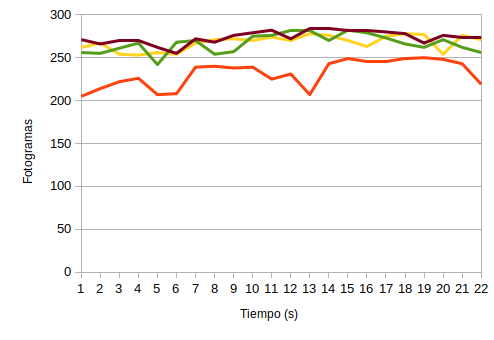
\includegraphics[width=0.435\textwidth]{performance/diagrama_gauss_fps_rec}
  		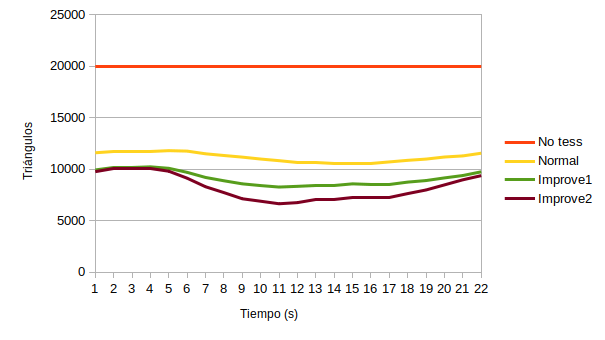
\includegraphics[width=0.555\textwidth]{performance/diagrama_gauss_triangulos}
  		\caption{Gráfica de la animación de rotación en gauss.in}
  		\label{fig:diagramas_gauss}
	\end{figure}
	
	\newpage
	\begin{center}
	\begin{tabular}{ | p{2cm} | | p{2cm} | p{2cm} | p{2cm} | p{2cm} | p{2cm} | }
		\hline
		\multicolumn{6}{ | c | } {waves.in}\\
		\hline
		$ $ &
		\multicolumn{5}{ | c | } {FPS}\\
		\hline
		Modo & Min & Max & Media & Mejora (fps) & Mejora ($\%$) \\
		\hline
		No tess.    & $21$ & $24$ & $21,81$ & $-$ & $-$ \\
		Normal tess. & $53$ & $63$ & $58,27$ & $+36,45$ & $+167,08$ \\
		Improve1 & $\boldsymbol{63}$ & $72$ & $64,68$ & $+42,86$ & $+196,45$ \\
		Improve2 & $62$ & $\boldsymbol{87}$ & $\boldsymbol{69,86}$ & $\boldsymbol{+48.04}$ & $\boldsymbol{+220,20}$ \\
		\hline
		$ $ &
		\multicolumn{5}{ | c | } {Triángulos}\\
		\hline
		Modo & Min & Max & Media & Mejora (tri.) & Mejora ($\%$) \\
		\hline
		No tess.    & $1000000$ & $1000000$ & $1000000,00$ & $-$ & $-$ \\
		Normal tess.    & $456480$ & $637537$ & $550527,77$ & $-449472,22$ & $-44,94$ \\
		Improve1 & $197244$ & $224222$ & $212327,00$ & $-787673,00$ & $-78,76$ \\
		Improve2 & $\boldsymbol{194703}$ & $\boldsymbol{223824}$ & $\boldsymbol{210390,31}$ & $\boldsymbol{-789609,68}$ & $\boldsymbol{-78,96}$ \\
		\hline
	\end{tabular}
	\end{center}
	\begin{figure}[h]
  		\centering
  		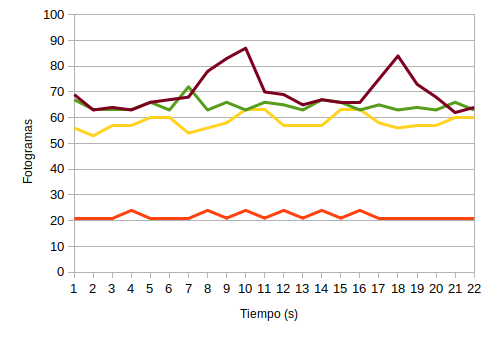
\includegraphics[width=0.435\textwidth]{performance/diagrama_waves_fps_rec}
  		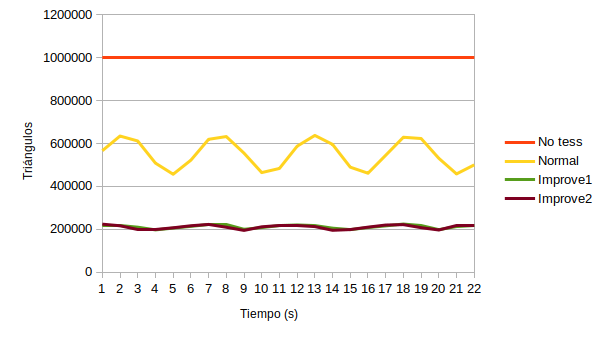
\includegraphics[width=0.555\textwidth]{performance/diagrama_waves_triangulos}
  		\caption{Gráfica de la animación de rotación en waves.in}
  		\label{fig:diagramas_waves}
	\end{figure}
	
	
	\newpage
	Las siguientes imágenes corresponden con la parametrización ``gaussiana.in'' con los distintos modos de visualización, donde para cada modo se ha buscado la configuración óptima, es decir, aquella en la que se ve visualmente bien y el nº de triángulos es mínimo. Por tanto, las $4$ imágenes debería ser exactamente iguales:
	\begin{figure}[h]
		\begin{minipage}{0.48\textwidth}
  			\centering
  			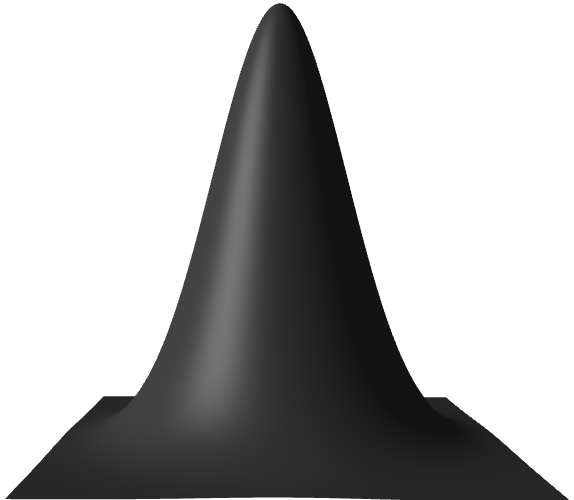
\includegraphics[width=0.9\textwidth]{performance/gauss_notess}
  			\caption{gaussiana.in sin teselar}
		\end{minipage}\hfill
		\begin{minipage}{0.48\textwidth}
  			\centering
  			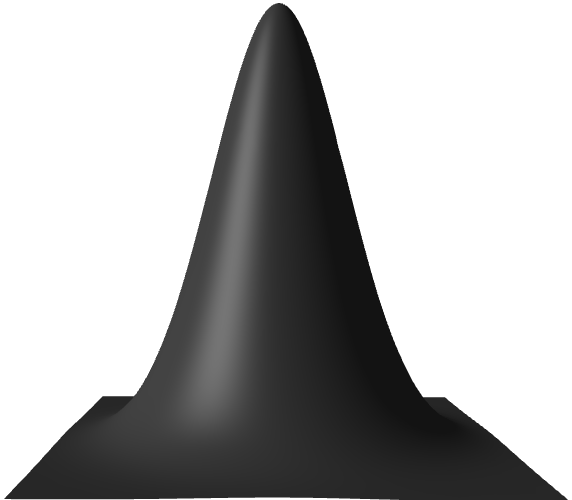
\includegraphics[width=0.9\textwidth]{performance/gauss_tessbad}
  			\caption{gaussiana.in teselado normal}
		\end{minipage}\hfill
		
		\begin{minipage}{0.48\textwidth}
  			\centering
  			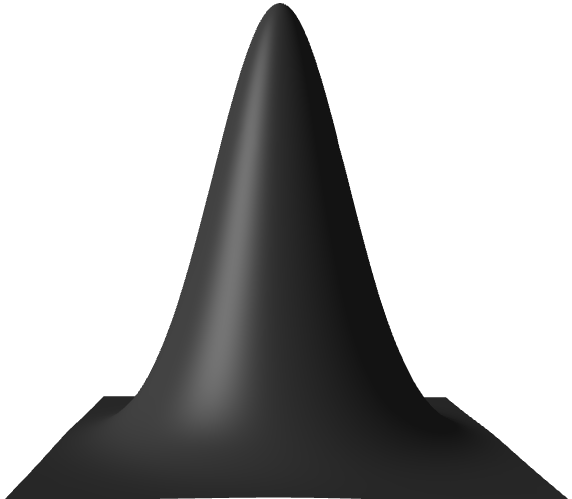
\includegraphics[width=0.9\textwidth]{performance/gauss_improve1}
  			\caption{gaussiana.in improve$1$}
		\end{minipage}\hfill
		\begin{minipage}{0.48\textwidth}
  			\centering
  			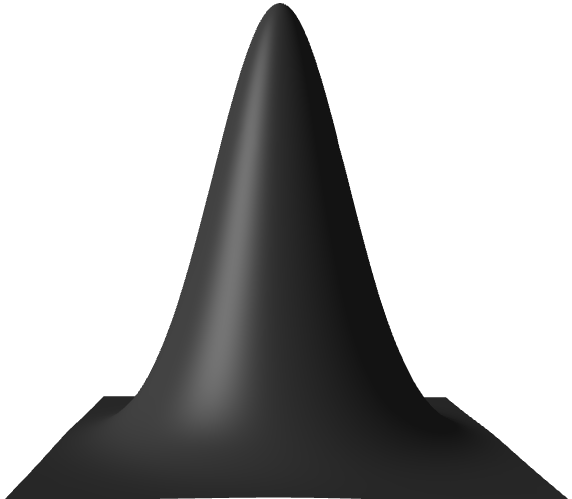
\includegraphics[width=0.9\textwidth]{performance/gauss_improve2}
  			\caption{gaussiana.in improve$2$}
		\end{minipage}\hfill
  		\label{fig:imagenes_gauss}
	\end{figure}	
	
	\newpage
	\begin{figure}[h]
		\begin{minipage}{0.48\textwidth}
  			\centering
  			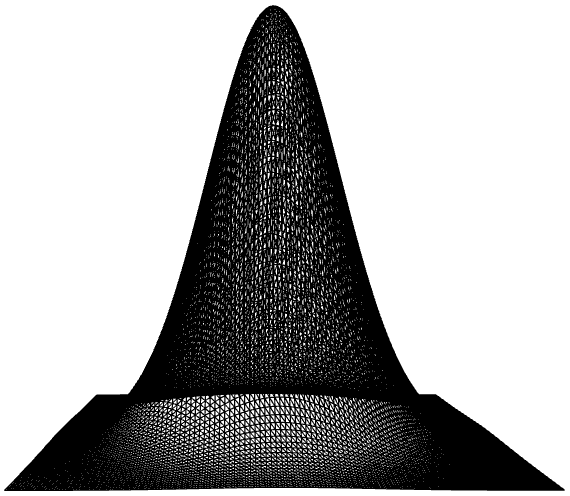
\includegraphics[width=0.9\textwidth]{performance/gauss_pol_notess}
  			\caption{gaussiana.in sin teselar}
		\end{minipage}\hfill
		\begin{minipage}{0.48\textwidth}
  			\centering
  			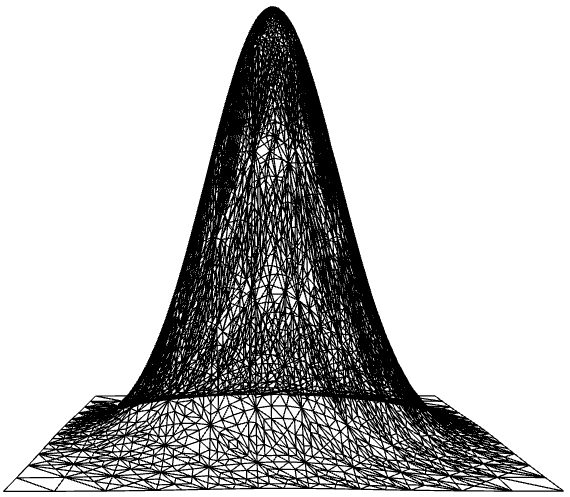
\includegraphics[width=0.9\textwidth]{performance/gauss_pol_tessbad}
  			\caption{gaussiana.in teselado normal}
		\end{minipage}\hfill
		
		\begin{minipage}{0.48\textwidth}
  			\centering
  			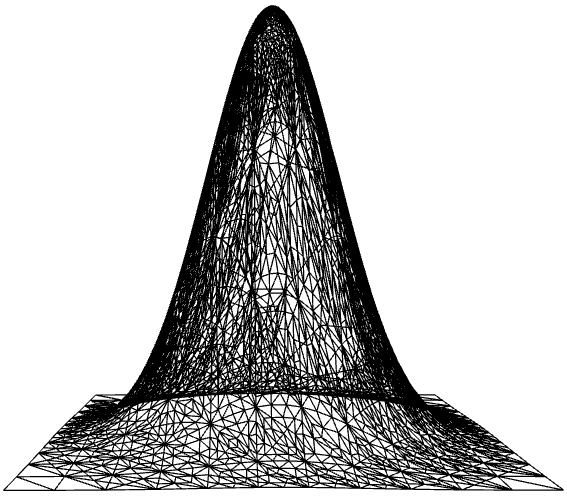
\includegraphics[width=0.9\textwidth]{performance/gauss_pol_improve1}
  			\caption{gaussiana.in improve$1$}
		\end{minipage}\hfill
		\begin{minipage}{0.48\textwidth}
  			\centering
  			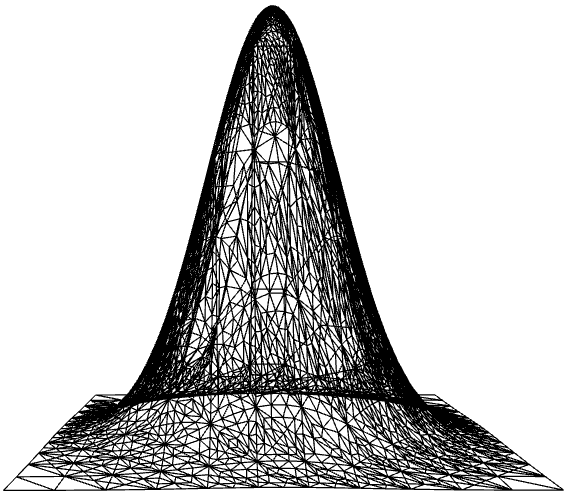
\includegraphics[width=0.9\textwidth]{performance/gauss_pol_improve2}
  			\caption{gaussiana.in improve$2$}
		\end{minipage}\hfill
  		\label{fig:imagenes_gauss_pol}
	\end{figure}	
	
	Seguidamente se muestran las imagenes correspondientes a la parametrización ``waves.in''. Sin embargo, debido a la complejidad de la superficie base (plano horizontal perturbado con un coseno), para el modo ``sin teselado'' es imposible llegar a una buena representación incluso utilizando una malla inicial de $1$ millón de triángulos, debido a la aparición de efectos ópticos, por la uniformidad de la malla inicial (parece haber más de un foco mientras que sólo hay uno).\\
	\\También es posible observar que al pasar de ``improve$1$'' a ``improve$2$'' puede aparecer algún segmento sin teselar. Se debe a que detecta que es un segmento oculto, mediante un cálculo basado en los extremos del segmento, pero como ya se comentó anteriormente esta funcionalidad está pensada para superficies específicas.
	\newpage
	\begin{figure}[h]
  		\centering
  		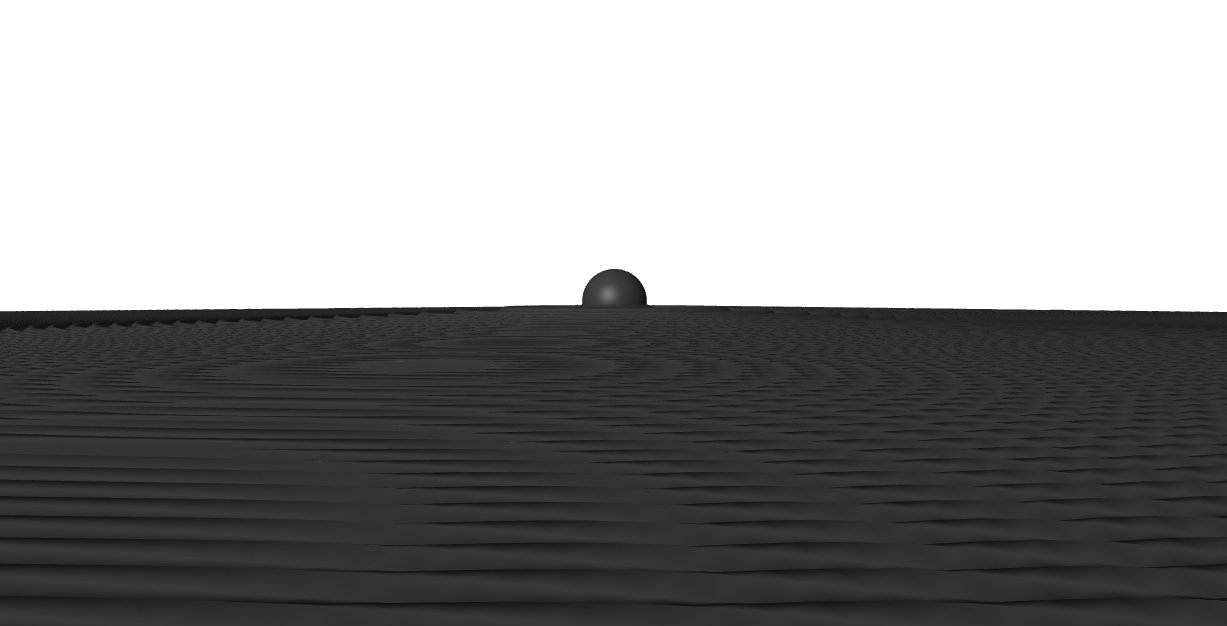
\includegraphics[width=0.9\textwidth]{performance/waves_notess}
  		\caption{waves.in sin teselar}
  		\vspace{0.5cm}
  		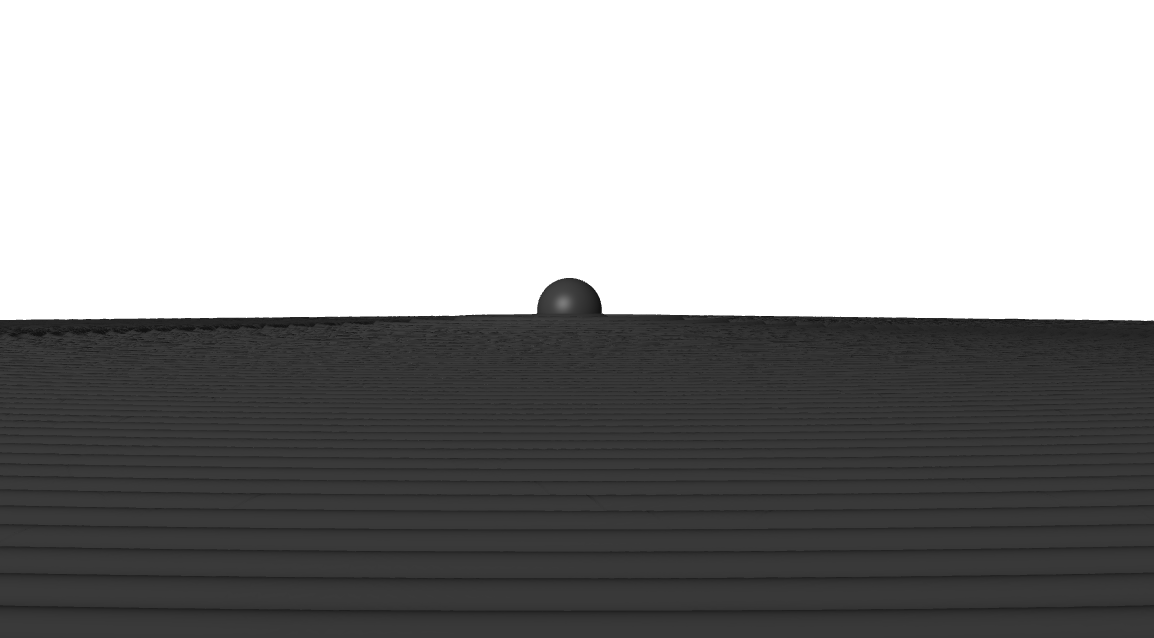
\includegraphics[width=0.9\textwidth]{performance/waves_tessbad}
  		\caption{waves.in teselado normal}
  		\vspace{0.5cm}
  		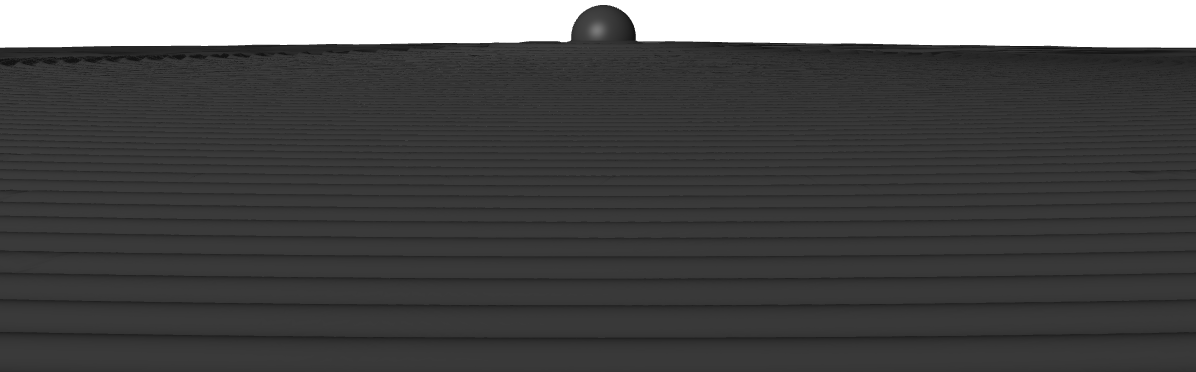
\includegraphics[width=0.9\textwidth]{performance/waves_improve1}
  		\caption{waves.in improve$1$}
  		\vspace{0.5cm}
  		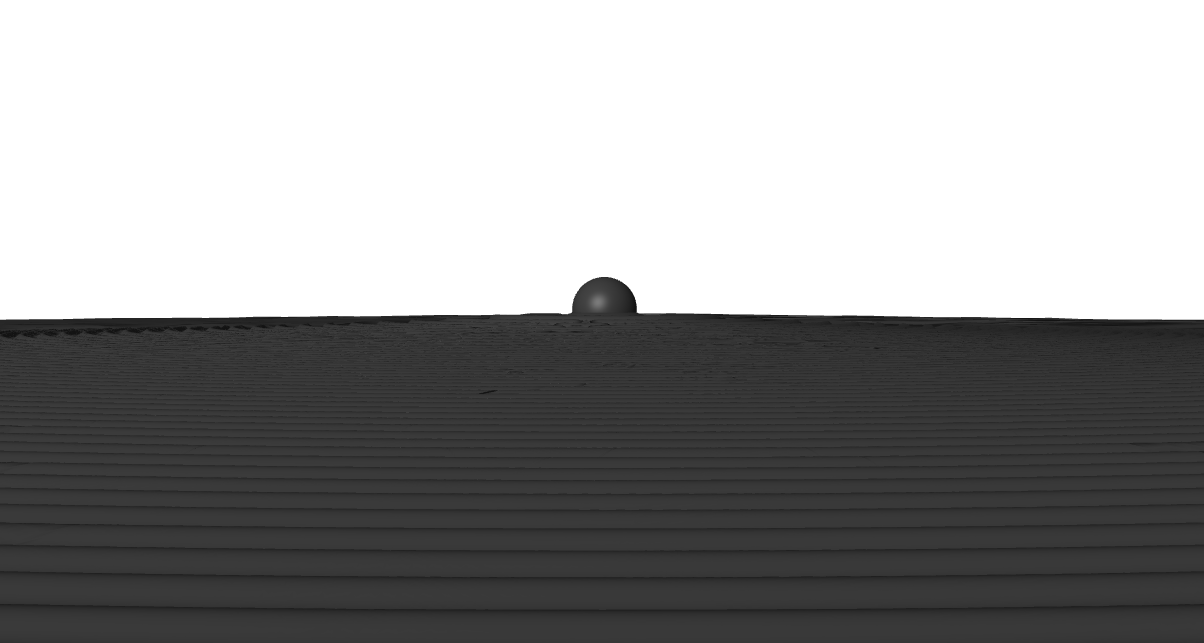
\includegraphics[width=0.9\textwidth]{performance/waves_improve2}
  		\caption{waves.in improve$2$}
  		\label{fig:imagenes_waves}
	\end{figure}	
	\begin{figure}[h]
  		\centering
  		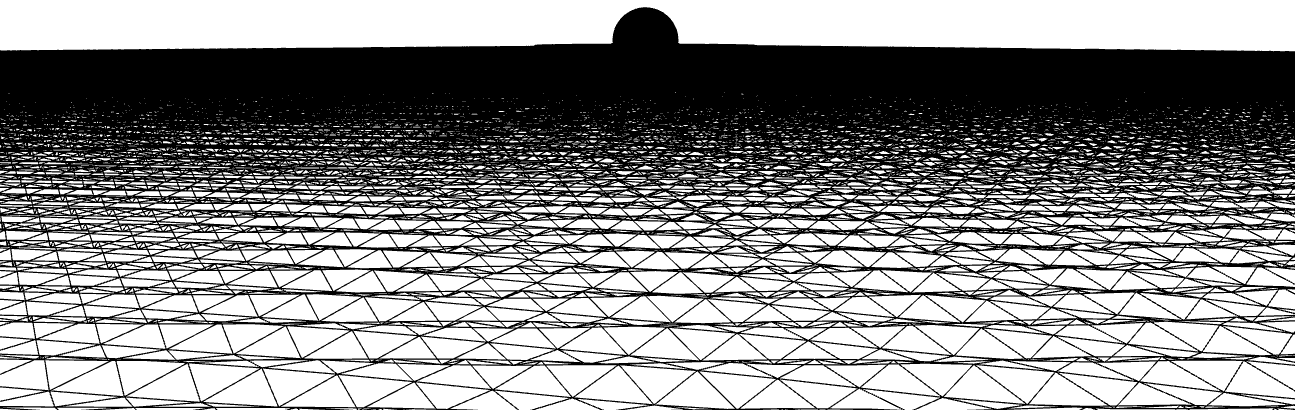
\includegraphics[width=0.9\textwidth]{performance/waves_pol_notess}
  		\caption{waves.in sin teselar}
  		\vspace{0.5cm}
  		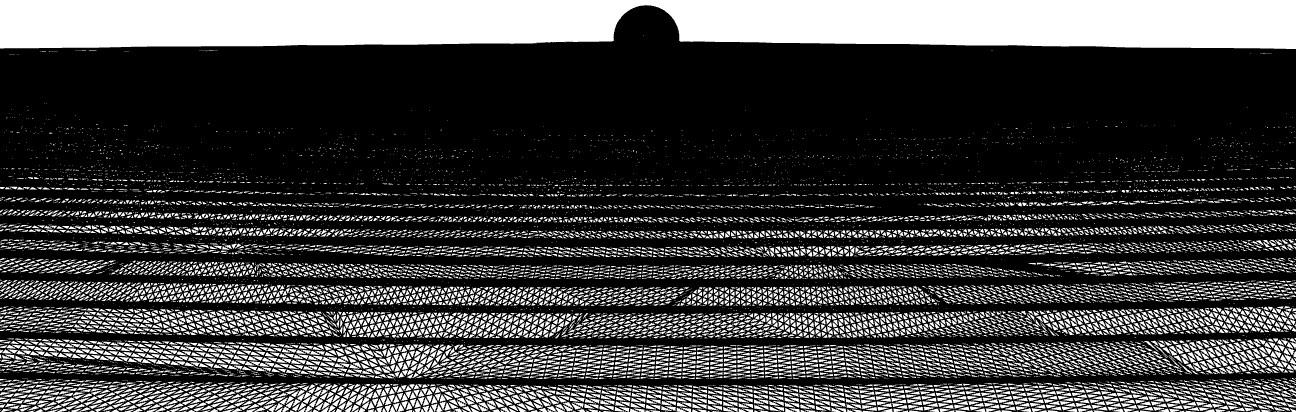
\includegraphics[width=0.9\textwidth]{performance/waves_pol_tessbad}
  		\caption{waves.in teselado normal}
  		\vspace{0.5cm}
  		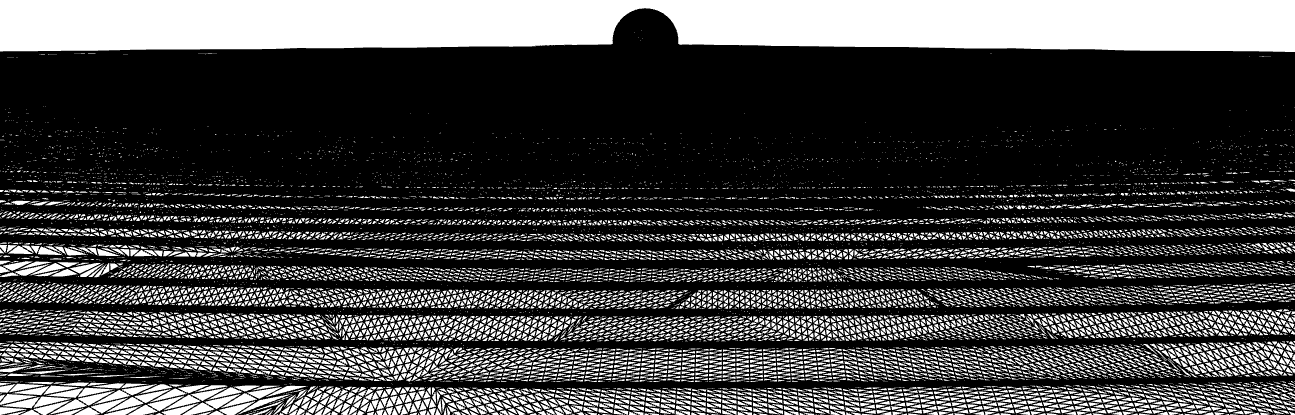
\includegraphics[width=0.9\textwidth]{performance/waves_pol_improve1}
  		\caption{waves.in improve$1$}
  		\vspace{0.5cm}
  		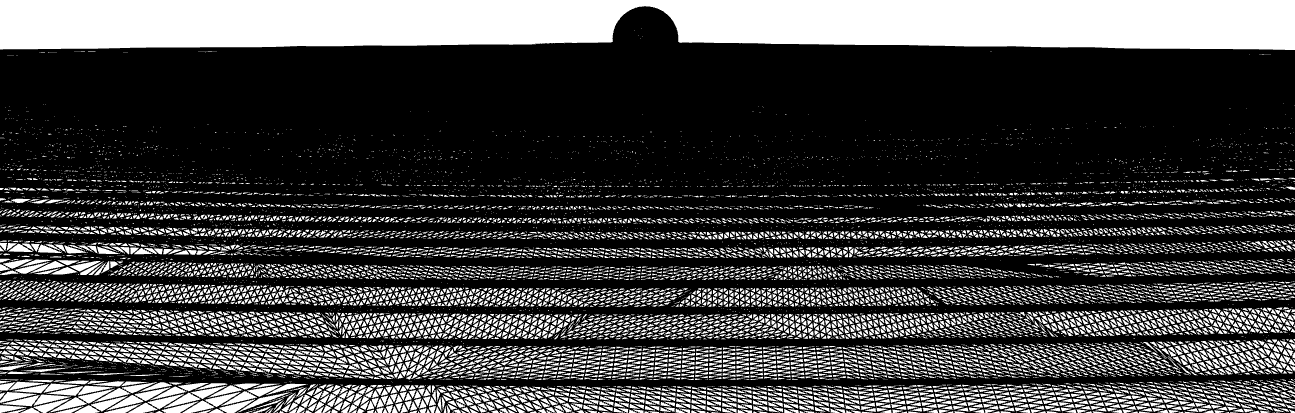
\includegraphics[width=0.9\textwidth]{performance/waves_pol_improve2}
  		\caption{waves.in improve$2$}
  		\label{fig:imagenes_waves_pol}
	\end{figure}	
	\newpage
		
		
\endinput
%------------------------------------------------------------------------------------
% FIN DEL CAPÍTULO. 
%------------------------------------------------------------------------------------


% --------------------------------------------------------------------
% APPENDIX: Opcional
% --------------------------------------------------------------------

\appendix % Reinicia la numeración de los capítulos y usa letras para numerarlos
\pdfbookmark[-1]{Apéndices}{appendix} % Alternativamente podemos agrupar los apéndices con un nuevo \part{Apéndices}

%% !TeX root = ../libro.tex
% !TeX encoding = utf8

\chapter{Primer apéndice}\label{ap:apendice1}

Los apéndices son opcionales.

Archivo: \texttt{apendices/apendice01.tex}

\endinput
%------------------------------------------------------------------------------------
% FIN DEL APÉNDICE. 
%------------------------------------------------------------------------------------

% !TeX root = ../libro.tex
% !TeX encoding = utf8

\chapter{Instalación del software}\label{ap:apendice1}

Los apéndices son opcionales.

Archivo: \texttt{apendices/guia\_instalacion.tex}

\endinput
%------------------------------------------------------------------------------------
% FIN DEL APÉNDICE. 
%------------------------------------------------------------------------------------

% !TeX root = ../libro.tex
% !TeX encoding = utf8

\chapter{Guía de uso del programa}\label{ap:apendice2}

En este capítulo se explicará brevemente cómo utilizar el programa. Aun así, la interfaz del programa se ha intentado diseñar lo más sencilla y clara posible, mostrando adicionalmente cuadros de texto si se mantiene el ratón sobre ciertos elementos.\\
\\Primero iniciaremos el programa tal y como se indica en el apéndice de \textbf{Instalación del software}. Una vez abierto el programa se mostrará siempre la última parametrización compilada existosamente. En el lateral izquierdo aparecerá un elemento de la interfaz, el menú, donde se podrá:
\begin{itemize}
	\item Parametrización:
	\begin{itemize}
		\item Seleccionar una parametrización ya existente, crearla o compilarla. También se podrá editar la actual, en cuyo caso aparecerá una ventana de edición de la propia interfaz. Dicha ventana también aparecerá en caso de que hayan errores léxicos, sintácticos o semánticos en la parametrización, con la salida del error desplegada.
		\item Cambiar el tamaño de la malla de partida, requeriendo su posterior actualización manual (botón contiguo).
		\item Visualizar la ventana con los parámetros temporales, con un tick que indica si está activa la ventana o no. Estará semi-visible si la superficie no tiene parámetros temporales. Dicha ventana mostrará los parámetros temporales en orden, permitiendo moverlos manualmente o generar una animación:
		\begin{itemize}
			\item Sin: movimiento sinusoidal entre el valor $0$ y $1$. Ideal para animaciones oscilantes.
			\item Lineal: movimiento lineal del valor $0$ al $1$, volviendo instantáneamente al $0$. Utilizado para movimientos lineales respecto al tiempo, que junto con el uso de funciones periódicas se puede generar la sensación de movimiento infinito (como los ejemplos wavesX.in).
		\end{itemize}
	\end{itemize}
	\item Visualización del objeto:
	\begin{itemize}
		\item Invertir normales (si no se quiere modificar la parametrización).
		\item Visualizar en modo malla (``Poligon mode'').
		\item Activar/desactivar la auto-rotación (rotación entorno al punto hacia el que mira la cámara).
		\item Ver los vectores tangentes, bitangentes y normales a los puntos (ya sean los de la malla inicial o de todos los generados).
		\item Cambiar modo del color de la superficie, ya sea el color base, la curvatura de Gauss, el área diferencial, la altura o los puntos críticos de ésta vista como función de Morse. Una vez seleccionado un modo, aparecerán coeficientes que permitirán ajustar correctamente la visualización a la superficie actual.
	\end{itemize}
	\item Opciones del teselado:
	\begin{itemize}
		\item Desactivar/activar el teselado.
		\item Indicar la precisión a la que se desea llegar con el teselado.
		\item Opciones avanzadas: modificar aquellos coeficientes específicos del teselado, como el tipo de mejora de rendimiento a usar (``improve'' normal o específica), la distancia de teselado, el umbral para detectar bordes y el exponente aplicado a la curvatura de Gauss. Todos ellos se inician con un valor por defecto.
	\end{itemize}
	\item Iluminación: es posible cambiar los coeficientes del modelo de iluminación ``Phong'' y ver el vector de dirección de la luz actualmente. La luz no es direccional, el vector indica la dirección de la luz con respecto al origen $(0,0)$.
	\item Estadísticas: muestra los fotogramas por segundo y la latencia medias, junto con el número de primitivas generadas tras la fase del geometry shader (después del tessellation shader). Permite además grabar los datos y los almacena de manera automática tras 22 segundos (antes si pulsamos ``Stop'' y seguidamente ``Save info'') en un fichero en el directorio raíz, con nombre dependiente de la parametrización y configuración actual.
\end{itemize}

\endinput
%------------------------------------------------------------------------------------
% FIN DEL APÉNDICE. 
%------------------------------------------------------------------------------------

% Añadir tantos apéndices como sea necesario 

% --------------------------------------------------------------------
% CONCLUSIONES
% --------------------------------------------------------------------

% !TeX root = ../libro.tex
% !TeX encoding = utf8
%
%*******************************************************
% Introducción
%*******************************************************

% \manualmark
% \markboth{\textsc{Introducción}}{\textsc{Introducción}} 

\chapter*{Conclusiones}
\addcontentsline{toc}{chapter}{Conclusiones} % Añade el glosario a la tabla de contenidos

De acuerdo con la comisión de grado, el TFG debe incluir una introducción en la que se describan claramente los objetivos previstos inicialmente en la propuesta de TFG, indicando si han sido o no alcanzados, los antecedentes importantes para el desarrollo, los resultados obtenidos, en su caso y las principales fuentes consultadas.

Ver archivo \texttt{preliminares/conclusiones.tex}

\endinput


% --------------------------------------------------------------------
% GLOSARIO: Opcional
% --------------------------------------------------------------------

% !TeX root = ../libro.tex
% !TeX encoding = utf8

\chapter*{Glosario}
\addcontentsline{toc}{chapter}{Glosario} % Añade el glosario a la tabla de contenidos

La inclusión de un glosario es opcional.

Archivo: \texttt{glosario.tex}

\begin{description} 
  \item[$\mathbb{R}$] Conjunto de números reales.

  \item[$\mathbb{C}$] Conjunto de números complejos.

  \item[$\mathbb{Z}$] Conjunto de números enteros.
\end{description}
\endinput
 

% -------------------------------------------------------------------
% BACKMATTER
% -------------------------------------------------------------------

%\backmatter % Desactiva la numeración de los capítulos
\pdfbookmark[-1]{Referencias e Índices}{BM-Referencias}


% BIBLIOGRAFÍA
%-------------------------------------------------------------------

\nocite{*}
\setbibpreamble{Las referencias se listan por orden alfabético. Aquellas referencias con más de un autor están ordenadas de acuerdo con el primer autor.\par\bigskip}
\bibliographystyle{alpha} 
\begin{small} % Normalmente la bibliografía se imprime en un tamaño de letra más pequeño.
\bibliography{library.bib}
\end{small}


% ÍNDICE TERMINOLÓGICO  (Opcional) 
%------------------------------------------------------------------- 

\cleardoublepage 
\begin{footnotesize} % Normalmente el índice se imprime en un tamaño de letra más pequeño.
\printindex 
\end{footnotesize}

\end{document}
